% !TeX spellcheck = lt
\documentclass{VUMIFPSbakalaurinis}
\usepackage{algorithmicx}
\usepackage{algorithm}
\usepackage{algpseudocode}
\usepackage{amsfonts}
\usepackage{amsmath}
\usepackage{bm}
\usepackage{caption}
\usepackage{color}
\usepackage{float}
\usepackage{graphicx}
\usepackage{listings}
\usepackage{url}
\usepackage{wrapfig}
\usepackage[table,xcdraw]{xcolor}
\usepackage[backend=biber]{biblatex}
\usepackage{enumitem}\setlist{nosep}
\usepackage{csquotes}
\usepackage{setspace}
\usepackage[hidelinks]{hyperref} 
\usepackage{subcaption}
\usepackage{hyperref}
\usepackage{listings}
\usepackage{xcolor}
\usepackage[utf8]{inputenc}
\usepackage[table,xcdraw]{xcolor}
\usepackage{longtable}
\usepackage{booktabs}
\usepackage{multirow}
\usepackage{pifont}
\usepackage{amssymb}
\usepackage{array}
\usepackage{hhline}
\usepackage{lscape}

\gappto{\UrlBreaks}{\UrlOrds}

\definecolor{codegreen}{rgb}{0,0.6,0}
\definecolor{codegray}{rgb}{0.5,0.5,0.5}
\definecolor{codepurple}{rgb}{0.58,0,0.82}
\definecolor{backcolour}{rgb}{0.95,0.95,0.92}

\lstdefinestyle{mystyle}{
	backgroundcolor=\color{backcolour},   
	commentstyle=\color{codegreen},
	keywordstyle=\color{magenta},
	numberstyle=\tiny\color{codegray},
	stringstyle=\color{codepurple},
	basicstyle=\ttfamily\footnotesize,
	breakatwhitespace=false,         
	breaklines=true,                 
	captionpos=b,                    
	keepspaces=true,                 
	numbers=left,                    
	numbersep=5pt,                  
	showspaces=false,                
	showstringspaces=false,
	showtabs=false,                  
	tabsize=4,
	prebreak=\raisebox{0ex}[0ex][0ex]{\ensuremath{\hookleftarrow}}
}

\lstset{style=mystyle}

\newcommand{\cmark}{\textcolor[HTML]{008000}{\ding{51}}}%
\newcommand{\xmark}{\textcolor[HTML]{800000}{\ding{55}}}%

\newcolumntype{P}[1]{>{\centering\arraybackslash}p{#1}}

%\onehalfspacing

% Titulinio aprašas
\university{Vilniaus universitetas}
\faculty{Informatikos institutas}
\department{Programų sistemos}
%\papertype{Bakalauro darbas}
\papertype{Bakalauro baigiamasis darbas}
\title{Skatinamojo mokymosi algoritmų skirtų Sokoban žaidimo agento valdymui palyginimas}
\titleineng{Comparison of Reinforcement Learning Algorithms for Sokoban Game Agent Training}
\author{Jokūbas Rusakevičius}
\supervisor{vyresn. m.d. Virginijus Marcinkevičius}
\reviewer{j. asist. Linas Petkevičius}
\date{Vilnius – \the\year}

\setmainfont{Palemonas}
\bibliography{bibliografija}

\begin{document}
\maketitle
\setcounter{page}{2}

\sectionnonumnocontent{}
\vspace{7cm}
\begin{center}
Dėkoju šeimai ir draugams, už meilę ir nuolatinį palaikymą bei darbo vadovui, vyresn. m.d. Virginijui Marcinkevičiui, už visapusišką pagalbą geriausio sprendimo beieškant.
\end{center}


\sectionnonumnocontent{Santrauka}
Šiame darbe buvo tiriamas Skatinamojo mokymosi agento pritaikymas Sokoban žaidimui. Darbe, aprašoma skatinamojo mokymosi teorija, pagrindiniai principai ir taikymo technikos. Taip pat, aprašomi skirtingi neuroniniai tinklai, dėl jų naudojimo skatinamojo mokymosi strategijų architektūroje. Darbe apžvelgiamos Sokoban žaidimo aplinkos ir modernios skatinamojo mokymosi bibliotekos, karkasai. Darbe lyginamos skirtingų skatinamojo mokymosi algoritmų implementacijos ir skirtingos strategijos Sokoban žaidimo aplinkoje. Darbe pritaikytas mokymosi žinių perdavimo principas apmokant skatinamojo mokymosi agentus žaisti sudėtingesnes Sokoban žaidimo aplinkas. Gauti žinių perdavimo taikymo rezultatai yra palyginami su agentu apmokytu vienodo sudėtingumo aplinkoje be žinių perdavimo. Išanalizuoti gauti rezultatai parodė, kad naudojant mokymosi žinių perdavimą Sokoban žaidimo aplinkai, skatinamojo mokymosi algoritmai gali pasiekti geresnių rezultatų.
\raktiniaizodziai{Skatinamasis mokymas, Sokoban žaidimas, aktoriumi-kritiku paremti metodai, žaidimo agento mokymas, mokymosi žinių perdavimas}   

\sectionnonumnocontent{Summary}
In this thesis, the application of the reinforcement learning agent to the Sokoban game was investigated. The paper describes the theory, basic principles and application techniques of reinforcement learning. Also, different neural networks are described, due to their use in the architecture of reinforcement learning strategies. Thesis reviews Sokoban game environments and state-of-art reinforcement learning libraries, frameworks. The paper compares implementations of different reinforcement learning algorithms and different strategies in the Sokoban game environment. The obtained results of transfer learning are compared to those of an agent trained in an environment of equal complexity without transfer learning. Analysis of the results showed that using transfer learning for the Sokoban game environment, reinforcement learning algorithms can achieve better results.
\keywords{reinforcement learning, Sokoban game, actor-critic based methods, game agent training, transfer learning}

\tableofcontents

\sectionnonum{Įvadas}\label{sec:ivadas}
{
	Šiame skyriuje aprašomi bakalauro darbo problematika, tikslas ir uždaviniai.
}
\subsectionnonum{Problematika}\label{subsec:problematika}
{
	Kompiuterių pajėgumui ir atliekamų operacijų per sekundę skaičiui nuolatos didėjant -- didėja ir lūkesčiai bei sprendžiamų uždavinių sudėtingumas. Dar reliatyviai neseniai sudėtingiausios programos ir kompiuterių sprendžiami uždaviniai susidėjo iš skaičiuotuvo operacijų ar žinučių perdavimo. Tačiau technologijoms tobulėjant, kiekvienam žmogui kišenėje besinešiojant pirmųjų kompiuterių kaip \enquote{ENIAC} \cite{computer_history} dydį pajuokiančius kompiuterinius įrenginius, natūraliai didėja ir jiems keliami iššūkiai.\par
	
	Šiais laikais kompiuteriai gali simuliuoti atominius sprogimus, nuspėti orus ir atlikti kitas didžiulių skaičiavimo išteklių reikalaujančias užduotis \cite{supercomputers}. Tačiau užduoties sudėtingumą gali lemti ne tik milžiniškų išteklių skaičiaus reikalavimas. 2016 metais matėme, kaip \enquote{Google’s AlphaGo} nugalėjo pasaulio aukščiausio lygio \enquote{Go} žaidėją ir čempioną Ke Jie \cite{go}. Autonominiai gatvėmis važinėjantys automobiliai neišvengiamai artėja, o \enquote{Boston Dynamics} robotai stebina savo galimybėmis \cite{bostondynamics}.\par
	
	Šie uždaviniai nėra trivialiai aprašomi ar išsprendžiami, jiems gali net neegzistuoti sprendimas. Tokiems uždaviniams spręsti yra naudojami mašininio mokymosi metodai (pvz. neuroniniai tinklai). Viena šių metodų paradigmų yra skatinamasis mokymas -- agento atliekami veiksmai yra reguliariai vertinami ir atitinkamai agentas yra apdovanojamas arba baudžiamas.\par
	
	Žaidimai dėl lengvai išskiriamų gerų ir blogų veiksmų, natūraliai, tampa pagrindine skatinamojo mokymosi algoritmų treniravimosi ir žaidimų aikštele. Klasikiniai Atari žaidimai yra dažnas tyrimų objektas \cite{mnih2013playing}. Tačiau žaidimų sudėtingumas varijuoja ir ne visus žaidimus kompiuteriai gali išmokti ar mokosi vienodai. Egzistuoja žaidimų ir uždavinių kategorijų, kurios skatinamojo mokymosi agentams yra ypatingai sudėtingos. Galimybė padaryti nepataisomą klaidą arba poreikis mąstyti į priekį yra tai, ko trūksta dažnam skatinamojo mokymosi agentui.\par
	
	Sokoban žaidimas būtent ir priklauso: sudėtingų išmokti kompiuteriui žaidimų kategorijai. Tai yra senas ir savo laiku dažnas mokslinių tyrimų objektas \cite{culberson1997sokoban, dor1999sokoban, junghanns1998sokoban, schaul2005evolving}. Tačiau nepaisant galvosūkio amžiaus, tai vis dar yra aktuali skatinamojo mokymosi taikymo aplinka. Sokoban žaidimas priklauso planavimo uždavinių kategorijai, kurie, dėl savo dažnai reikalingo gebėjimo mąstyti į priekį, yra sunkiai išsprendžiami skatinamojo mokymosi būdu \cite{SchraderSokoban2018}.\par
}
\subsectionnonum{Darbo tikslas}\label{subsec:tikslas}
{
	Šio darbo \textbf{tikslas} -- palyginti skatinamojo mokymosi algoritmus, siekiant nustatyti efektyviausią algoritmą ir jo strategiją Sokoban žaidimui.
}
\subsectionnonum{Darbo uždaviniai}\label{subsec:uzdaviniai}
{
	Darbui iškelti \textbf{uždaviniai}:
	\begin{enumerate}
		\item Atlikti skatinamojo mokymosi algoritmų analizę ir atrinkti keletą potencialiausių algoritmų Sokoban žaidimo agento mokymui.
		\item Paruošti eksperimentinę aplinką Sokoban žaidimui.
		\item Atlikti eksperimentą, siekiant nustatyti, kuri Sokoban žaidimo agento valdymo strategija yra geriausia.
		\item Eksperimentiškai palyginti skatinamojo mokymosi algoritmus: A2C, ACER, PPO naudojant mažiausią įmanomą Sokoban žaidimo aplinką.
		\item Panaudoti žinių perdavimą, siekiant Sokoban žaidimo agentą apmokyti veikti sudėtingesnėse aplinkose.
	\end{enumerate}
}
\section{Skatinamasis mokymas ir dirbtiniai neuroniniai tinklai}\label{sec:1}
Šiame skyriuje aprašyta teorinė bakalauro darbo dalis.

\subsection{Skatinamasis mokymasis}\label{subsec:RL} 
{
	Skatinamasis mokymasis (\textit{angl. reinforcement learning}) (RL), kartu su prižiūrimuoju ir neprižiūrimuoju mokymu, yra viena iš pagrindinių mašininio mokymosi (ML) paradigmų. Klasikinis RL modelis susideda iš agento (\textit{angl. agent}), kuris priima sprendimus ir atlieka veiksmus (\textit{angl. actions}) pagal strategiją  (\textit{angl. policy}), paremtus aplinkos būsena (\textit{angl. state}), ir siekiantis pasiekti didžiausią įmanomą atlygį (\textit{angl. reward}) (paveikslėlis~\ref{img:rl}).\par
	
	\begin{figure}[H]
		\centering
		
\includegraphics[scale=0.33]{img/rl}
		\caption{Skatinamojo mokymosi agento sąveika su aplinka}
		\label{img:rl}
	\end{figure} 
	
	Skirtingai nei kitos ML paradigmos, RL sprendžia ne regresijos, klasifikacijos, ar grupavimo, bet atlygiu paremtas (\textit{angl. reward-based}) problemas, ir tai daro bandymų ir klaidų (\textit{ang. trial and error}) principu. Dėmesys yra nukreiptas ne į sužymėtas (\textit{angl. labeled}) įvesties ir išvesties duomenų poras, bet į balanso tarp tyrinėjimo (\textit{angl. exploration}) ir išnaudojimo (\textit{angl. exploitation}) ieškojimą \cite{kaelbling_littman_moore}.\par
	
	\begin{figure}[H]
		\centering
		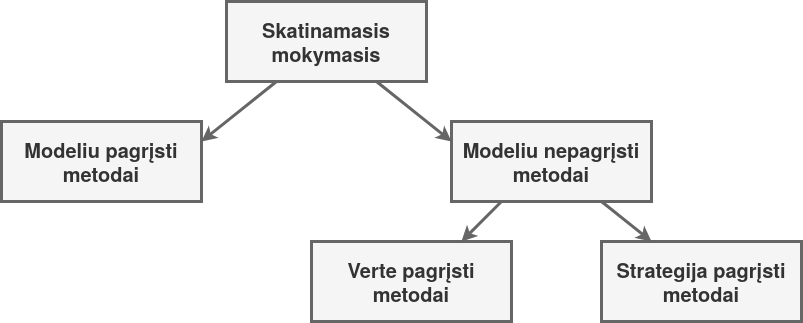
\includegraphics[scale=0.33]{img/rl_overview}
		\caption{Skatinamojo mokymosi algoritmų kategorijos}
		\label{img:rl_overview}
	\end{figure} 
	
	RL algoritmai yra skirstomi pagal skirtingus rodiklius į kelias skirtingas kategorijas \cite{kindsOfRlAlgorithms} (paveikslėlis~\ref{img:rl_overview}). Prieš aiškinantis kuo skiriasi kiekviena kategorija, svarbu suprasti, kad RL algoritmai susideda iš dviejų fazių:
	
	\begin{enumerate}
		\item \textbf{Mokymosi fazė} -- (\textit{angl. learning phase}) tai yra algoritmo apmokymo dalis, kai kiekvienas agento priimtas sprendimas ir atliktas veiksmas aplinkoje bei gautas atlygis ir nauja aplinkos būsena yra panaudojama tolimesniam modelio optimizavimui ir gerinimui.
		\item \textbf{Taikymo fazė} -- (\textit{angl. interface phase}) tai yra algoritmo dalis, kai, nepriklausomai nuo atlikto veiksmo optimalumo, modelis nebėra keičiamas ir yra naudojamos iki šiol išmoktos reikšmės.
	\end{enumerate}

	 Kaip jau minėta anksčiau, RL algoritmai yra skirstomi į skirtingas kategorijas (paveikslėlis~\ref{img:rl_overview}). Pagal modelio struktūrą \cite{kindsOfRlAlgorithms}:
	 
	\begin{enumerate}
		\item \textbf{Pagrįsti modeliu} -- (\textit{angl. model-based}) tai yra algoritmai, kurie optimalios strategijos apskaičiavimui naudojasi transakcijų funkcija (ir atlygio funkcija) (daugiau punkte~\ref{subsubsec:MDP}). Pagrįsti modeliu algoritmai gali nuspėti galimus aplinkos pakitimus, kadangi naudojasi apskaičiuota transakcijų funkcija. Tačiau, modelio turima funkcija gali būti tik apytikslė \enquote{tikrajai} funkcijai, tad modelis gali niekada nepasiekti optimalaus sprendimo. 
		\item \textbf{Nepagrįsti modeliu} -- (\textit{angl. model-free}) tai yra algoritmai, kurie apskaičiuodami optimalią strategija nesinaudoja ir nebando apskaičiuoti aplinkos dinamikų (transakcijų ir perėjimų funkcijos nenaudojamos). Nepagrįsti modeliu algoritmai bando apskaičiuoti vertės arba strategijos funkciją tiesiai iš patirties (interakcijų su aplinka).
	\end{enumerate}

	Pagal strategijos pritaikymą:
	
	\begin{enumerate}
		\item \textbf{Besiremiantys optimalia strategija} -- (\textit{angl. on-policy}) algoritmai, kurie, mokymosi metu rinkdamiesi veiksmą, remiasi strategija išvesta iš tuo metu apskaičiuotos optimaliausios strategijos bei atlieka atnaujinimus remdamiesi ta pačia strategija.
		\item \textbf{Nesiremiantys optimalia strategija} -- (\textit{angl. off-policy}) algoritmai, kurie mokymosi metu remiasi skirtinga strategija nei tuo metu apskaičiuota optimaliausia strategija. Atnaujinimai atliekami remiantis geresnį rezultatą gražinančia strategija.
	\end{enumerate}

	Nepagrįsti modeliu algoritmai yra skirstomi į dar dvi kategorijas, pagal tai, kuo jie yra pagrįsti:
	
	\begin{enumerate}
		\item \textbf{Pagrįsti verte} -- (\textit{angl. value-based}) tai yra algoritmai pagrįsti \textit{laiko skirtumų mokymusi} (\textit{angl. temporal difference learning}), kur yra mokomasi funkcija \(V^{\pi}\)  arba \(V^*\) (daugiau punkte~\ref{subsubsec:rlTeorija}).
		\item \textbf{Pagrįsti strategija} -- (\textit{angl. policy-based}) tai algoritmai, kurie tiesiogiai mokosi optimalios strategijos \(\pi^*\) arba bando apytiksliai surasti optimalią strategiją.
	\end{enumerate}

	Toliau šiame poskyryje bus giliau nagrinėjamas RL ir jį sudarantys elementai.
}
\subsubsection{Skatinamojo mokymosi bendroji teorija} \label{subsubsec:rlTeorija} 
{
	Šiame darbe bus remiamasi standartine RL aplinka, kur agentas yra aplinkoje \(\mathcal{E}\) diskretų kiekį laiko vienetų arba žingsnių (\textit{angl. time steps}). Kiekvieną žingsnį \(t\) agentas gauna informaciją apie aplinkos būseną \(s_t\) ir iš visų įmanomų veiksmų rinkinio \(\mathcal{A}\) pasirenka atitinkamą veiksmą \(a_t\) pagal strategiją \(\pi\), kur strategija \(\pi\) pasako kokį veiksmą \(a_t\) rinktis situacijoje \(s_t\). Aplinka agentui grąžina informaciją apie sekančią aplinkos būseną \(s_{t+1}\) ir skaliarinę atlygio reikšmę \(r_t\). Toks procesas yra tęsiamas, kol aplinka pasiekia galinę būseną (\textit{angl. terminal state}). Kai galinė būsena yra pasiekiama -- procesas yra pradedamas iš naujo. Rezultatas \(R_t = \sum_{k=0}^{\infty} \gamma^k r_{t+k}\) yra bendras žingsnyje \(t\) surinktas atlygis su nuolaidos koeficientu (\textit{angl. discount factor}) \(\gamma \in (0, 1] \). Agento tikslas yra gauti didžiausia įmanoma tikėtina rezultatą su visomis aplinkos būsenomis \(s_t\).\par
	
	Veiksmo vertė (\textit{angl. action value}) apskaičiuojama: \(Q^{\pi}(s, a) = \mathbb{E}[R_t|s_t = s, a] \), kur tikėtinas rezultatas \(\mathbb{E}\) gaunamas pagal strategiją \(\pi\) pasirinkus veiksmą \(a\), esant situacijoje \(s\). Optimali vertės funkcija \(Q^*(s, a) = \max_{\pi}Q^{\pi}(s, a)\), grąžina didžiausią strategijos \(\pi\) pasiektą veiksmo vertę aplinkos būsenai \(s\) ir veiksmui \(a\). Panašiai, aplinkos būsenos \(s\) vertė (\textit{angl. state value}) remiantis strategija \(\pi\) yra apibrėžiama taip: \(V^{\pi}(s) = \mathbb{E}[R_t|s_t = s] \), ir tai yra tikėtinas rezultatas būsenai \(s\) pagal strategiją \(\pi\).\par
	
	Verte ir modeliu pagrįstuose (poskyris~\ref{subsec:RL}) RL metoduose, veiksmo vertės funkcija yra reprezentuojama funkcijos aproksimacija (\textit{angl. approximtator}), pavyzdžiui, neuroniniu tinklu (daugiau poskyryje~\ref{subsec:neuro}). Jei imame \(Q(s, a; \theta)\) kaip apytikslė veiksmo vertės funkciją su parametrais \(\theta\), tada atnaujinimai skirti \(\theta\) gali būti išvesti iš įvairių RL algoritmų. Pavyzdžiui, vienas tokių algoritmų gali būti Q-mokymasis (\textit{angl. Q-learning}), kurio tikslas yra tiesiogiai surasti apytikslę optimalią veiksmo vertės funkciją: \(Q^*(s, a) \approx Q(s, a; \theta)\). Vieno-žingsnio (\textit{angl. one-step}) Q-mokymosi algoritmuose vertės funkcijos \(Q(s, a; \theta)\) parametrai \(\theta\) yra išmokstami iteraciškai mažinant nuostolių (\textit{angl. loss}) funkcijos seką, kur kiekviena \(i\)-toji nuostolių funkcija yra funkcija~(\ref{eq:loss}) ir \(s'\) yra būsena pasiekta po būsenos \(s\).
	\begin{equation}\label{eq:loss}
		L_i(\theta_i) = \mathbb{E} \left( r + \gamma \max_{a'} Q(s', a'; \theta_{i-1}) - Q(s, a; \theta_i) \right)^2
	\end{equation}
	
	Vieno-žingsnio Q-mokymosi algoritmas yra taip pavadintas, nes jo veiksmo vertės funkcija \(Q(s, a)\) yra atnaujinama link vieno-žingsnio rezultato \(r + \gamma \max\limits_{a'} Q(s', a'; \theta) \). Vienas vieno-žingsnio metodo naudojimo trūkumas yra, kad gautas atlygis \(r\) paveikia tik tiesiogiai į jį atvedusią būsenos ir veiksmo porą \(s\), \(a\). Kitų būsenų ir veiksmų porų vertės paveikiamos tik netiesiogiai per atnaujintą \(Q(s, a)\) vertę. Tai gali lemti labai lėtą mokymosi procesą, kadangi reikia labai daug atnaujinimų paskleisti (\textit{angl. propagate}) atlygį į aktualias ankstesnes būsenas ir veiksmus.\par
	
	Vienas būdas paskleisti atlygį greičiau yra naudoti \(n\)-žingsnių (\textit{angl. \(n\)-step}) rezultatus \cite{watkins, peng_williams_1994}. Naudojant \(n\)-žingsnių Q-mokymosi algoritmą, \(Q(s, a)\) yra atnaujinama link \(n\)-žingsnių rezultato, apibrėžto: \(r_t + \gamma r_{t+1} + \cdots + \gamma^{n-1} r_{t+n-1} + \max\limits_a \gamma^n Q(s_{t+n}, a) \). Taip pasiekiama, kad vienas atlygis \(r\) tiesiogiai paveikia \(n\) ankstesnių būsenų ir veiksmų porų reikšmes ir gaunamas potencialiai daug efektyvesnis aktualioms būsenos-veiksmo poroms atlygio skleidimo procesas.\par
	
	Atvirkščiai nei verte pagrįsti metodai, strategija pagrįsti ir modeliu nepagrįsti (poskyris~\ref{subsec:RL}) RL metodai tiesiogiai parametrizuoja strategiją \(\pi(a|s;\theta)\) ir atnaujina parametrus \(\theta\) atlikdami apytikslį gradiento padidinimą (\textit{angl. gradient ascent}) \(\mathbb{E}[R_t]\). Vienas tokio metodo pavyzdys yra REINFORCE šeimos algoritmai \cite{williams_1992}. Standartinis REINFORCE atnaujina strategijos parametrus \(\theta\) kryptimi \(\nabla_\theta \log \pi(a_t|s_t; \theta)R_t\), kas yra nešališkas (\textit{angl. unbiased}) \(\nabla_\theta \mathbb{E}[R_t] \) apskaičiavimas. Taip pat, yra įmanoma sumažinti šio apskaičiavimo dispersiją (\textit{angl. variance}) išlaikant nešališkumą iš rezultato atimant išmoktą būsenos funkciją \(b_t(s_t)\), žinomą kaip bazė (\textit{angl. baseline}) \cite{williams_1992}. Gautas gradientas yra \(\nabla_\theta \log \pi(a_t|s_t; \theta)(R_t - b_t(s_t))\).\par
	
	Vertės funkcijos išmoktas apskaičiavimas yra dažnai naudojamas kaip bazė \(b_t(s_t) \approx V^\pi(s_t) \) vedanti link daug mažesnės strategijos gradiento dispersijos. Kai apytikslė vertės funkcija yra naudojama kaip bazė, skaičius \(R_t - b_t\) gali būti panaudotas \textit{pranašumo} (\textit{angl. advantage}) apskaičiavimui veiksmui \(a_t\) būsenoje \(s_t\) arba \(A(a_t, s_t) = Q(a_t, s_t) - V(s_t)\), nes \(R_t\) yra \(Q^\pi (a_t, s_t)\) apskaičiavimas ir \(b_t\) yra \(V^\pi(s_t)\) apskaičiavimas. Toks principas gali būti vadinamas aktoriaus-kritiko architektūra, kur strategija \(\pi\) yra aktorius ir bazė \(b_t\) yra kritikas \cite{rl_intro_book}.
}
\subsubsection{Markovo sprendimo priėmimo procesai}\label{subsubsec:MDP}
{ 
	Pirmieji aprašyti Markovo sprendimo priėmimo procesai (\textit{angl. Markov decision processes}, MDP) \cite{mdp} priminė Markovo grandines (\textit{angl. Markov chains}).\par
	
	\textbf{Markovo grandinė} -- tai kiekviename žingsnyje atsitiktinai judantis iš vienos į kitą būseną (\textit{angl. state}) procesas su fiksuotu skaičiumi būsenų, kur tikimybė pereiti iš būsenos \(s\) į būseną \(s'\) yra taip pat fiksuota ir priklauso tik nuo poros \((s, s')\), ne nuo jau praėjusių būsenų. Markovo grandinės neturi atminties \cite{handson}. 
	
	\begin{figure}[H]
		\centering
		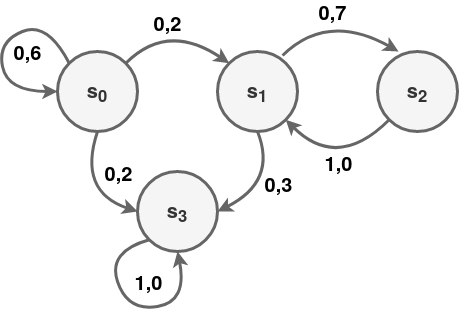
\includegraphics[scale=0.33]{img/markov_chain}
		\caption{Markovo grandinės pavyzdys}
		\label{img:markovChain}
	\end{figure} 
	
	Paveikslėlyje~\ref{img:markovChain} pavaizduotas Markovo grandinės pavyzdys su keturiomis būsenomis. Jeigu laikome būseną \(s_0\) pradine, tai yra \(70\%\) tikimybė, kad procesas pasiliks šioje būsenoje ir kitą žingsnį. Po tam tikro kiekio žingsnių, procesas galiausiai paliks \(s_0\) ir niekada nebegrįš į šią būseną, nes jokia kita rodyklė nerodo į \(s_0\). Jei procesas pereis į būseną \(s_1\), tai yra labiausiai tikėtina (\(60\%\) tikimybė), jog kita būsena bus \(s_2\)) ir tada iškart atgal į \(s_1\) (\(100\%\) tikimybė). Procesas gali pereiti per \(s_1\) \(s_2\) kelis kartus, prieš galiausiai patenkant į galinę būseną \(s_3\), kur procesas ir pasiliks.\par
	
	MDP nuo Markovo grandinės skiriasi tuo, kad MDP perėjimai iš vienos būsenos į kitą, gali turėti jiems priskirtus atlygius (gali būti teigiami ir neigiami). RL problemos labai dažnai yra formuluojamos kaip MDP, kur agento tikslas yra surasti strategija, kuri privestų prie didžiausio bendro atlygio per trumpiausia laiko tarpą \cite{handson}.\par
	
	\begin{figure}[H]
		\centering
		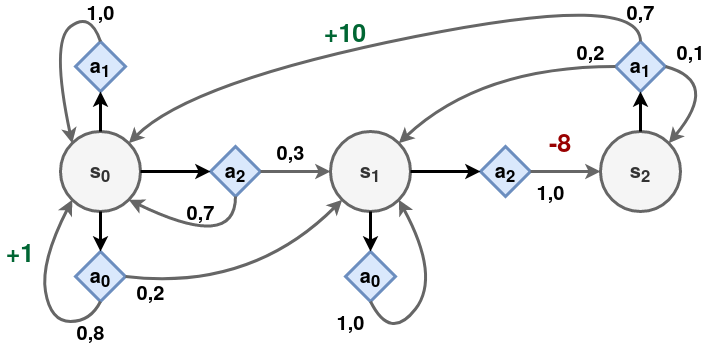
\includegraphics[scale=0.33]{img/mdp}
		\caption{Markovo proceso pavyzdys}
		\label{img:mdp}
	\end{figure} 
	
	Paveikslėlyje~\ref{img:mdp} pavaizduotas MDP pavyzdys su trimis būsenomis ir iki trijų diskrečių veiksmų per būseną. Jeigu laikome, kad agentas pradeda būsenoje \(s_0\), tai pirmame žingsnyje agentas gali pasirinkti vieną iš trijų galimų: \(a_0\), \(a_1\), \(a_2\) veiksmų. Jeigu agentas pasirinktų atlikti veiksmą \(a_1\) -- jis garantuotai liktų būsenoje \(s_0\). Tačiau, jeigu agentas pasirinktų veiksmą \(a_0\) -- yra \(80\%\) tikimybė, gauti atlygį \(+1\) ir likti toje pačioje būsenoje \(s_0\) arba \(20\%\) tikimybė be atlygio patekti į būseną \(s_1\). Galiausiai arba \(a_0\), arba \(a_2\) veiksmu agentas pateiks į būseną \(s_1\). Šioje būsenoje agentas gali pasirinkti tik vieną iš dviejų veiksmų: \(a_0\) arba \(a_2\). Nors yra du galimi veiksmai, tik veiksmas \(a_2\) veda į kitą būseną. Tačiau pasirinktus šį veiksmą agentas taip pat garantuotai gauna atlygį (bausmę) \(-8\). Pasiekus būseną \(s_3\) yra galimas tik vienas veiksmas \(a_1\), bet galimi trys skirtingi rezultatai: likti toje pačioje būsenoje \(s_3\) (\(10\%\) tikimybė), pereiti į būseną \(s_1\) (\(20\%\) tikimybė) arba grįžti į pradinę būseną \(s_0\) (\(70\%\) tikimybė) ir gauti atlygį \(+10\).\par
	
	Optimaliai būsenos vertei bet kuriai būsenai \(s\), žymimai \(V^*(s)\), nustatyti, galima naudoti Belmano Optimalumo Lygtį (\textit{angl. Bellman optimality equation}). Ši rekursyvi lygtis~(\ref{eq:bellmanOptimal}) parodo, kad jei agentas atlieka veiksmus optimaliai, tada optimali dabartinės būsenos reikšmė yra lygi vidutiniškai agento gaunamam atlygiui atlikus vieną optimalų veiksmą, plius visų įmanomų toliau einančių būsenų tikėtina optimali vertė.
	
	\begin{equation}\label{eq:bellmanOptimal}
		V^* = \max_a \sum_{s'}T(s, a, s')[R(s, a, s') + \gamma V^*(s')] \textrm{ su visais } s
	\end{equation} 
	
	\begin{itemize}
		\item \textbf{Transakcijų funkcija} (\textit{angl. transaction function}) \(T(s, a, s')\) yra perėjimo iš būsenos \(s\) į būseną \(s'\) tikimybė, agentui pasirinkus veiksmą \(a\).
		\item \textbf{Atlygio funkcija} (\textit{angl. reward function}) \(R(s, a, s')\) yra agento gaunamas atlygis, kai jis pereina iš būsenos \(s\) į būseną \(s'\), agentui pasirinkus veiksmą \(a\).
		\item \(\gamma\) yra nuolaidos koeficientas.
	\end{itemize}\par

	MDP taip pat gali būti užrašytas tokiu būdu: \(\mathcal{M} = (\mathcal{S}, \mathcal{A}, P, R, \gamma)\).
	\begin{itemize}
		\item \(\mathcal{S}\): visų būsenų rinkinys.
		\item \(\mathcal{A}\): visų veiksmų rinkinys.
		\item \(P : \mathcal{S} \times \mathcal{A} \times \mathcal{S} \rightarrow [0, 1]\): transakcijų tikimybės pasiskirstymas \(P(s'|s, a)\).
		\item \(R : \mathcal{S} \rightarrow \mathbb{R}\): atlygio funkcija, \(R(s)\) yra atlygis būsenai \(s\).
		\item \(\gamma\): nuolaidos koeficientas.
	\end{itemize}
}
\subsubsection{Sustiprinto mokymosi strategijos paieška}
{
	Agento naudojamas algoritmas veiksmo pasirinkimo sprendimui priimti yra vadinamas strategija. Strategija gali būti visiškai bet koks algoritmas, net nesvarbu ar jis yra stochastinis, ar deterministinis. Tačiau strategijos, kurios naudoja atsitiktines reikšmes yra vadinamos stochastinėmis strategijomis (\textit{angl. stochastic policy}). Kintamieji, naudojami strategijos sprendimo priėmimui vadinami strategijos parametrais (\textit{angl. policy parameters}) ir šių kintamųjų optimalių reikšmių ieškojimo procesas vadinamas strategijos paieška (\textit{angl. policy search}). Strategijos parametrų įmanomų reikšmių kombinacijų rinkinys vadinamas strategijos plotu (\textit{angl. policy space}) \cite{handson}.\par
	
	Atlikti strategijos paiešką galima įvairiais būdais. Jei strategijos paieškos plotas yra reliatyviai mažas ir ieškoma vieno ar dviejų parametrų reikšmės, galima pasitelkti paprasčiausią brutalią jėgą (\textit{angl. brute force}) ir išbandyti visus ar dauguma įmanomų variantų ir pasirinkti geriausią iš jų. Tačiau, paieškos plotui didėjant, gero strategijos parametrų rinkinio paieška sudėtingėja ir reikalingų resursų skaičius didėja eksponentiškai, todėl šitas sprendimas dažniausiai nėra taikomas.\par
	
	Kitas būdas yra pasitelkti genetinius algoritmus \cite{genetic_algorithm_book}. Sukuriant pirmąją kartą (\textit{angl. generation}) strategijų su atsitiktinai parinktais strategijos parametrais ir iteratyviai šalinant blogiausius rezultatus rodančias vienetus bei atliekant atsitiktines mutacijas geriausiai pasirodžiusiųjų kopijoms. Taip galima iteruoti \enquote{išgyvenusiųjų} ir jų \enquote{vaikų} kartas, kol pasiekiama tinkama strategija. \par
	
	Dar vienas sprendimas būtu naudoti optimizavimo metodus. Įvertinus atlygio gradientus, atsižvelgti į strategijos parametrus ir nežymiai juos pakeisti sekant gradientus link aukštesnio atlygio (gradiento pakilimas). Tai vadinama strategijos gradientais \cite{handson}.	
}
\subsubsubsection{Strategijos gradientai}
{
	Strategijos gradientai (\textit{angl. policy gradients}, PG) yra atsakingi už strategijos parametrų optimizavimą sekant aukštesnio atlygio link. REINFORCE algoritmas \cite{williams_1992} yra populiari PG klasė. Toliau aprašoma dažna variacija:
	
	\begin{enumerate}
		\item Neuroninio tinklo strategija sužaidžia žaidimą kelis kartus, apskaičiuoja kiekvieno žingsnio gradientus, kurie padidintų pasirinkto veiksmo pasirinkimo tikimybę ateityje, bet dar jų nepritaiko.
		\item Po kelių sužaistų epizodų, apskaičiuojami taškai kiekvienam veiksmui.
		\item Jei pasirinkto veiksmo atlygio taškai yra teigiami, reiškia tai buvo geras pasirinkimas ir anksčiau apskaičiuoti gradientai yra pritaikomi. Tačiau, jei veiksmo taškai yra neigiami, tada pritaikomi anksčiau apskaičiuotiems priešingi gradientai. Taip tinkamo veiksmo pasirinkimas tampa labiau tikėtinas ir netinkamo -- mažiau.
		\item Apskaičiuojamas visų galutinių gradientų vektorių vidurkis ir yra atliekamas Gradientų nusileidimo (\textit{angl. Gradient Descent}) žingsnis.
	\end{enumerate}
}
\subsubsection{Aktoriaus-kritiko principas}\label{subsubsec:actor-critic}
{
	Aktoriaus-kritiko (\textit{angl. actor-critic}) algoritmai yra algoritmų kategorija, kuri apjungia verte pagrįstus ir strategija pagrįstus algoritmus. Šios algoritmų kategorijos tikslas yra pasinaudoti abiejų principų pranašumais ir pašalinti jų trūkumus. Pagrindinė idėja yra padalinti modelį į dvi dalis: viena atsakinga už veiksmo suradimą duotajai būsenai, kita už veiksmo vertės įvertinimą \cite{rl_intro_book}.\par
	
	Aktoriaus įvestis yra aplinkos būsena (paveikslėlis, \ref{img:actor-critic}), o išvestis geriausias jai veiksmas. Aktorius mokydamasis optimalios strategijos yra atsakingas už agento elgesį (strategija pagrįstas). Kritikas vertina veiksmo pasirinkimą apskaičiuodamas vertės funkciją (verte pagrįstas). Abu modeliai dalyvauja žaidime ir laikui bėgant tampa geresni savo vaidmenyse. Gauta architektūra išmoksta žaisti žaidimą efektyviau nei abu metodai galėtų atskirai.
	
	\begin{figure}[H]
		\centering
		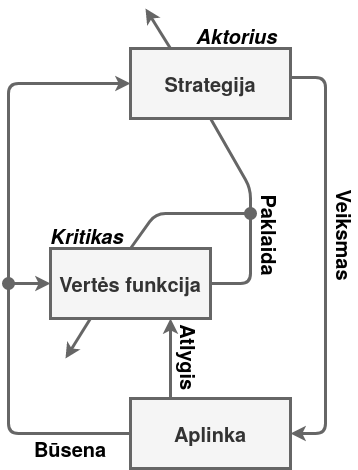
\includegraphics[scale=0.33]{img/actor-critic}
		\caption{Aktoriaus-kritiko schema}
		\label{img:actor-critic}
	\end{figure} 
}
\subsection{Dirbtiniai neuroniniai tinklai}\label{subsec:neuro}
{
	Dirbtiniai neuroniniai tinklai (\textit{angl. artificial neural networks}) (ANN) egzistuoja jau labai ilgą laiką, pirmos jų variacijo pristatytos dar 1943 metais \cite{mcculloch_pitts_1943}. Per tiek metu ANN implementacijos ir galimybės gerokai išaugo ir nors ANN perėjo per kelias populiarumo ir visiškos \enquote{užmiršties} epochas, yra matoma nemažai priežasčių, kodėl ši technologija turės ir turi didelę įtaką mūsų gyvenimams \cite{handson}. Keli pavyzdžiai:
	\begin{itemize}
		\item Dėl egzistuojančių didelių kiekių duomenų, kuriuos galima panaudoti ANN apmokymams bei dėl dažno ANN geresnių rezultatų nei kitos ML technikos pasiekimo naudojant sudėtingas ir labai dideles problemas.
		
		\item Dėl labai didelio kompiuterijos pasaulio patobulėjimo bei skaičiavimų galios išaugimo. 2000-2001 metais geriausiu laikytas superkompiuteris \enquote{ASCI White}\footnote{\url{https://www.top500.org/resources/top-systems/asci-white-lawrence-livermore-national-laboratory/}} galėjo pasiekti teoretinį 12.3 TFLOPS\footnote{TFLOPS arba teraFLOPS yra \(10^{12}\) FLOPS. FLOPS (\textit{angl. floating point operations per second}) yra operacijų atliekamų per sekundę su slankaus kablelio skaičiais matmuo dažnai naudojamas kompiuterinių įrenginių pajėgumui nustatyti.} pajėgumą, kai šiuolaikinės vartotojams prieinamos GPU yra vertinamos net iki 14\footnote{\url{https://www.microway.com/knowledge-center-articles/comparison-of-nvidia-geforce-gpus-and-nvidia-tesla-gpus/}} TFLOPS (ir nesveria šimtų tonų).
		
		\item Dėl dažno ANN pasiekiamų rezultatų atsiradimo žinių akiratyje, kas lemia didėjantį ir taip populiarų ANN technologijų finansavimą, greitėjantį progresą bei šią technologiją naudojančių naujų produktų atsiradimą\cite{handson}.
	\end{itemize}
	
Toliau šiame skyriuje bus rašoma apie ANN ir jų variacijas bei susijusias technologijas.
}
\subsubsection{Dirbtinių neuroninių tinklų architektūros komponentai}\label{subsubsec:components}
Šiame punkte aprašomi smulkūs ANN architektūros komponentai.

\subsubsubsection{Dirbtinis neuronas}\label{subsubsubsec:artificial_neurons}
{
	\textbf{Dirbtinis neuronas} (\textit{angl. artificial neuron}) -- paprastas biologinio neurono modelis, turintis vieną ar daugiau binarinių (įjungta/išjungta) įvesčių (ryšių) ir vieną binarinę išvestį. Dirbtinis neuronas aktyvuoja išvestį, kai tam tikras skaičius įvesčių yra aktyvus. Paveikslėlyje~\ref{img:artificial_neurons} pavaizduotas paprastas ANN, galintis atlikti įvairius loginius skaičiavimus, su sąlyga, kad neuronas aktyvuojamas, kai bent dvi įvestys yra aktyvios. Dirbtinis neuronas yra labai limituotas savo galimybėmis todėl sudėtingesnis neurono medelis yra reikalingas sudėtingėjant užduotims. 
	
	\begin{figure}[H]
		\centering
		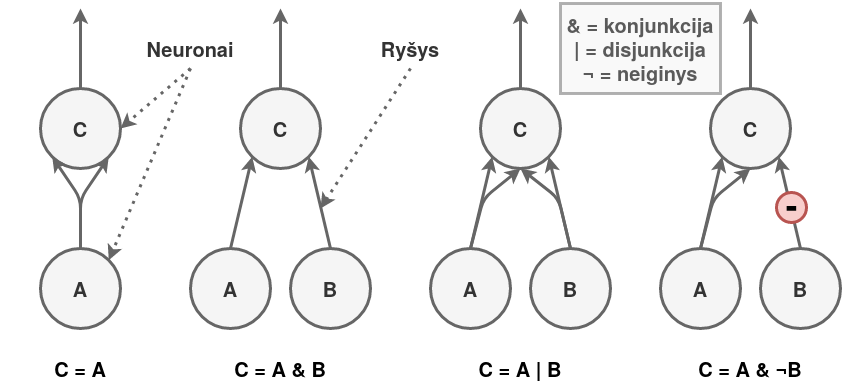
\includegraphics[scale=0.33]{img/artificial_neurons}
		\caption{Dirbtinio neurono atliekančio loginius skaičiavimus pavyzdys}
		\label{img:artificial_neurons}
	\end{figure} 
}
\subsubsubsection{Linijinis slenksčio vienetas}\label{subsubsubsec:ltu}
{
	\textbf{Linijinis slenksčio vienetas} (\textit{angl. linear treshold unit}, LTU) buvo pirmasis dirbtinis neuronas (papunktis~\ref{subsubsubsec:artificial_neurons}). LTU įvestys ir išvestys yra skaičiai (ne binarinės reikšmės) ir kiekviena įvestis turi savo svorį. LTU suskaičiuoja sumą su įvesčių svoriais (\(z = w_1 x_1 + w_2 x_2 + \cdots + w_n x_n = \mathbf{w}^T \cdot \mathbf{x} \)), tada suskaičiuotai sumai pritaiko žingsnio funkcija (\textit{angl. step function}) ir išveda rezultatą: \(h_\mathbf{w}(\mathbf{x}) = \textrm{žingsnis}(z) = \textrm{žingsnis}(\mathbf{w}^T \cdot \mathbf{x})\) (paveikslėlis~\ref{img:ltu}).
	
	\begin{figure}[H]
		\centering
		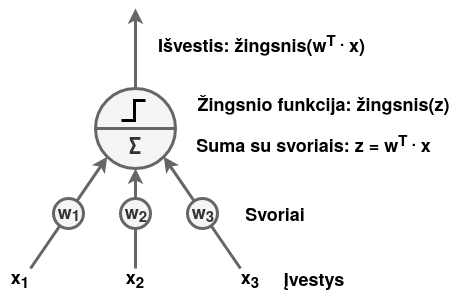
\includegraphics[scale=0.33]{img/ltu}
		\caption{Linijinis slenksčio vienetas}
		\label{img:ltu}
	\end{figure} 
}
\subsubsubsection{Pagalbiniai neuronai}\label{subsubsubsec:additional_neurons}
{
	Formuojant ANN neužtenka tik skaičiavimus atliekančių neuronų. Be LTU ir dirbtinio neurono egzistuoja keli paprasti pagalbiniai neuronai:\par
	
	\begin{itemize}
	\item \textbf{Įvesties neuronas} (paveikslėlis~\ref{img:input_neuron}) išveda tuos pačius duomenis, kurie yra jam paduodame per įvestį.
	
	\item \textbf{Postūmio neuronas} (paveikslėlis~\ref{img:bias_neuron}) neturi įvesties ir visada išveda tą pačią reikšmę (konstanta).
	\end{itemize}
	
	\begin{figure}[H]
		\centering
		\begin{subfigure}[b]{.5\textwidth}
			\centering
			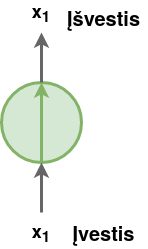
\includegraphics[scale=0.33]{img/input_neuron}
			\caption{Įvesties neuronas}
			\label{img:input_neuron}
		\end{subfigure}%
		\begin{subfigure}[b]{.5\textwidth}
			\centering
			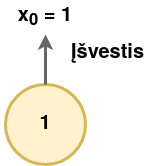
\includegraphics[scale=0.33]{img/bias_neuron}
			\caption{Postūmio neuronas}
			\label{img:bias_neuron}
		\end{subfigure}
		\caption{Pagalbiniai neuronai}
		\label{img:additional_neurons}
	\end{figure} 
}
\subsubsubsection{Dirbtinių neuroninių tinklų sluoksiniai}\label{subsubsubsec:neural_layers}
{
	Kiekvienas ANN yra sudaryti iš sluoksnių. Sluoksnis -- tai tame pačiame ANN gylyje kartu dirbančių neuronų rinkinys. Yra keli pagrindiniai apibrėžimai susiję su ANN sluoksniais: 
	
	\begin{itemize}
		\item \textbf{Įvesties sluoksnis} (\textit{angl. input layer}) -- tai pats pirmas sluoksnis ANN architektūroje. Dar vadinamas pereinamuoju (\textit{angl. passthrough}), nes visi šiam sluoksniui paduoti duomenys yra tiesiogiai perduodami į tolimesnį sluoksnį be jokių pakeitimų.
		
		\item \textbf{Išvesties sluoksnis} (\textit{angl. output layer}) -- tai paskutinis sluoksnis ANN architektūroje, atsakingas už bendrą viso tinklo išvestą rezultatą.
		
		\item \textbf{Paslėptasis sluoksnis} (\textit{angl. hidden layer}) -- taip ANN architektūroje vadinami visi tarp įvesties ir išvesties sluoksnių esantys sluoksniai.
	\end{itemize}
	
	Pagal paslėptųjų sluoksnių kiekį ANN architektūros yra klasifikuojamos į dvi grupes:
	
	\begin{itemize}
		\item \textbf{Negilusis neuroninis tinklas} (\textit{angl. shallow neural network}) -- tai klasė tinklų, kurių architektūra yra sudaryta tik iš įvesties ir išvesties sluoksnių bei nėra nei vieno paslėpto sluoksnio.
		
		\item \textbf{Gilusis neuroninis tinklas} (\textit{angl. deep neural network}) (DNN) -- tai klasė tinklų, kurių architektūroje be įvesties ir išvesties sluoksnių yra bent vienas paslėptas sluoksnis.
\end{itemize}
}
\subsubsection{Parceptronas}\label{subsubsec:perceptron}
{
	\textbf{Perceptronas} yra viena iš paprasčiausių ANN architektūrų ir yra paremta LTU (daugiau papunktis~\ref{subsubsubsec:ltu}) \cite{rosenblatt1957perceptron}. Perceptronuose dažniausiai naudojama sunkiosios pusės (\textit{angl. heaviside step}) žingsnio funkcija~(\ref{eq:heaviside}) arba kartai ženklo (\textit{angl. sign}) funkcija~(\ref{eq:sign}).
	
	\begin{align}
		\label{eq:heaviside}
		\textrm{heaviside} (z) = &
		\begin{cases} 
			0 & \textrm{jei} z < 0 \\ 
			+1 & \textrm{jei} z \geq 1 
		\end{cases} \\
		\label{eq:sign}
		\textrm{sign} (z) = &
		\begin{cases} 
			-1 & \textrm{jei} z < 0 \\ 
			0 & \textrm{jei} z = 0 \\ 
			+1 & \textrm{jei} z > 1 
		\end{cases}
	\end{align}
	
	Perceptronas sudarytas iš dviejų pilnai sujungtų sluoksnių (papunktis~\ref{subsubsubsec:neural_layers}): sluoksnio sudaryto tik iš LTU ir sluoksnio sudaryto iš įvesties neuronų bei dažnai papildomo postūmio neurono (\(x_0 = 1\)), kuris visada grąžina 1. Paveikslėlyje~\ref{img:perceptron} pavaizduotas perceptronas su dviem įvestimis ir trimis išvestimis (pavyzdžiui, galintis klasifikuoti į tris skirtingas klases).
	
	
	\begin{figure}[H]
		\centering
		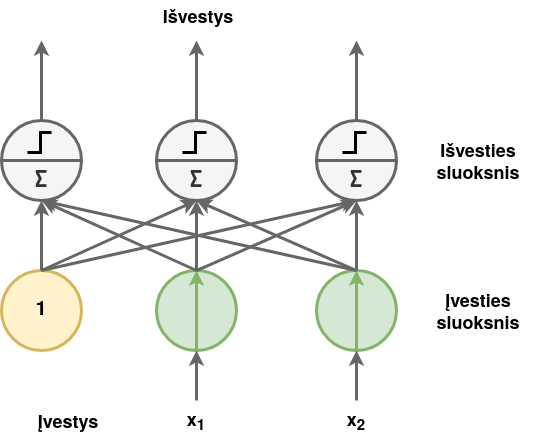
\includegraphics[scale=0.33]{img/perceptron}
		\caption{Perceptrono pavyzdys}
		\label{img:perceptron}
	\end{figure} 
	
	Perceptronai yra apmokomi naudojantis Hebo\footnote{(\textit{angl. Hebb's rule}) \enquote{Cells that fire together, wire together} svoriai tarp neuronų yra didinami, jei jie turi vienodą išvestį.} taisyklės variaciją, kuri atsižvelgia į tinklo padarytas klaidas ir mažina ryšių vedančių į neteisingą išvestį įtaką. Perceptrono mokymosi lygtis \(w_{i, j}^{\textrm{ktias žingsnis}} = w_{i, j} + \eta (\hat{y}_j - y_j)x_i\) susideda iš \(w_{i, j}\) yra ryšio svorio tarp \(i\)-tojo įvesties ir \(j\)-tojo išvesties neuronų, \(x_i\) \(i\)-tosios įvesties, \(\hat{y}_j\) \(j\)-tojo išvesties neurono išvesties, \(y_j\) \(j\)-tajo išvesties neurono išvesties tikslo reikšmės, bei \(\eta\) mokymosi greičio koeficiento.\par
}
\subsubsection{Daugiasluoksniai perceptronai}\label{subsubsec:mlp}
{
	Daugiasluoksniai perceptronai (\textit{angl. multi-layer perceptron}) (MLP) yra pilnai sujungtas DNN sudarytas iš: įvesties sluoksnio, vieno ar daugiau paslėptų sluoksnių sudarytų iš LTU ir išvesties sluoksnio, taip pat sudaryto iš LTU. Visi, išskyrus išvesties, sluoksniai taip pat turi po vieną postūmio neuroną. Paveikslėlyje~\ref{img:mlp} pavaizduotas dviejų įvesčių, trijų išvesčių ir vieno paslėptojo sluoksnio MLP.
	
	\begin{figure}[H]
		\centering
		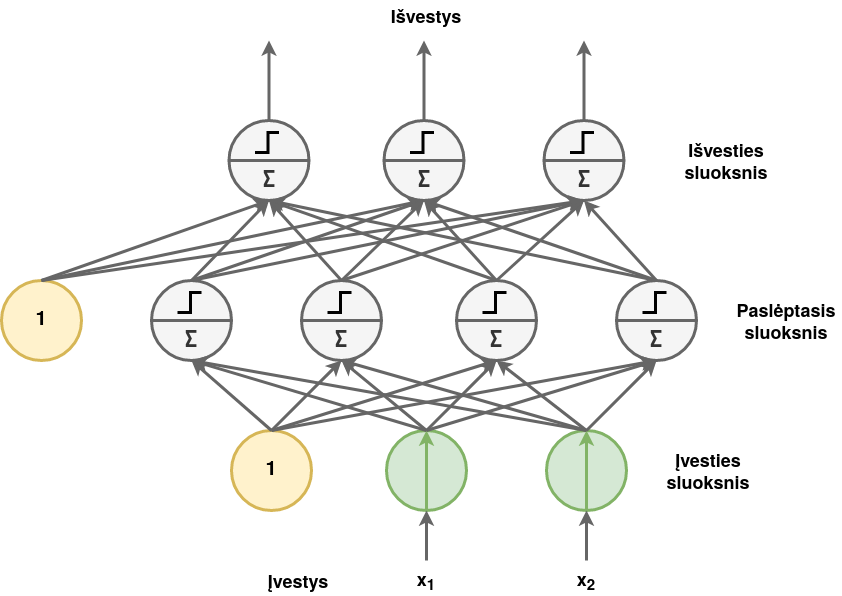
\includegraphics[scale=0.33]{img/mlp}
		\caption{Daugiasluoksnio perceptrono pavyzdys}
		\label{img:mlp}
	\end{figure} 
	
	MLP mokymui yra naudojamas atgalinio sklidimo (\textit{angl. backpropogation}) mokymo algoritmas \cite{rumelhart1985learning}, kai treniravimo metu pirma yra apskaičiuojama prognozė, išmatuojamas klaidingumas ir grįžtama atgal per sluoksnius apskaičiuojant kiekvieno sluoksnio įtaką gautam klaidingumui bei nežymiai keičiant ryšių svorius, ateities skaičiavimų klaidingumui sumažinti. Šiam procesui yra reikalingi gradientai, todėl MLP žingsnio funkcija yra pakeičiama į aktyvavimo funkciją (\textit{angl. activation function}). Populiariausios aktyvavimo funkcijos:
	
	\begin{itemize}
		\item \textbf{Logistinė funkcija} \(\sigma(z) = (1 + \exp(-z))^{-1}\), su visomis reikšmėmis turi stipriai apibrėžtą nenulinę išvestinę, kas leidžia progresuoti kiekviename mokymo žingsnyje (paveikslėlis~\ref{img:log_graph}).
		
		\item \textbf{Hiperbolinio tangento funkcija} \(\tanh(z) = 2\sigma(2z) – 1\), panašiai kaip logistinė funkcija yra S-formos, tačiau funkcijos galimos reikšmės yra \((–1, 1)\) ribose, kas padeda normalizuoti sluoksnių išvestis ir pagreitina konvergencija (paveikslėlis~\ref{img:tanh_graph}).
		
		\item \textbf{ReLU funkcija} \(\textrm{ReLU}(z) = \max(0, z)\), nors nėra diferencijuojama kai \(z=0\), praktiko pritaikyta veikia labai gerai. Didžiausias šios funkcijos privalumas -- labai greitas apskaičiavimas (paveikslėlis~\ref{img:relu_graph}).
	\end{itemize}
	
	
	\begin{figure}[H]
		\centering
		\begin{subfigure}[b]{.333\textwidth}
			\centering
			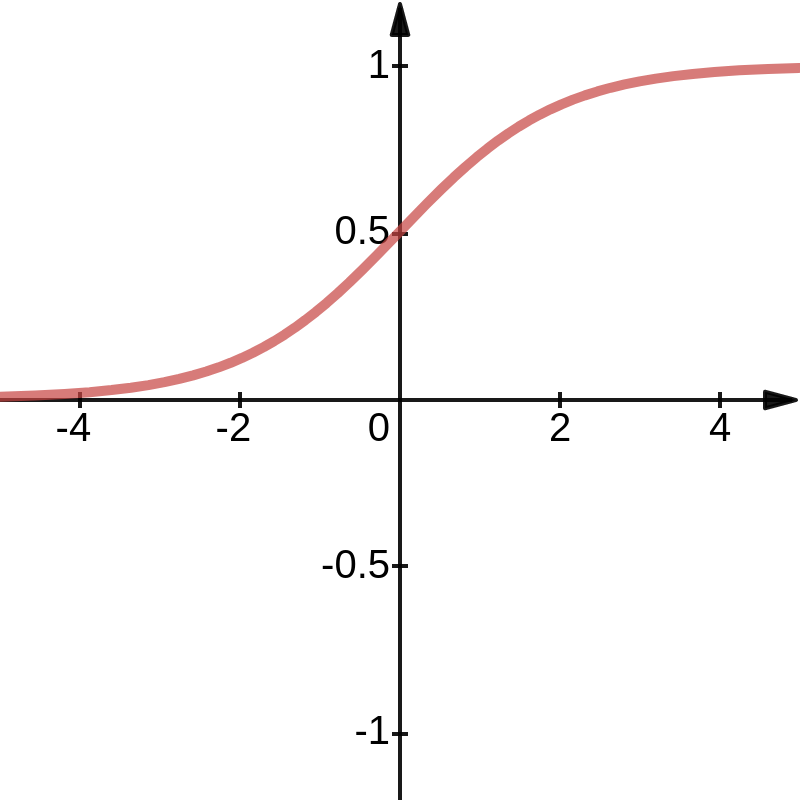
\includegraphics[width=.75\textwidth]{img/log_graph}
			\caption{Logistinė funkcija}
			\label{img:log_graph}
		\end{subfigure}%
		\begin{subfigure}[b]{.333\textwidth}
			\centering
			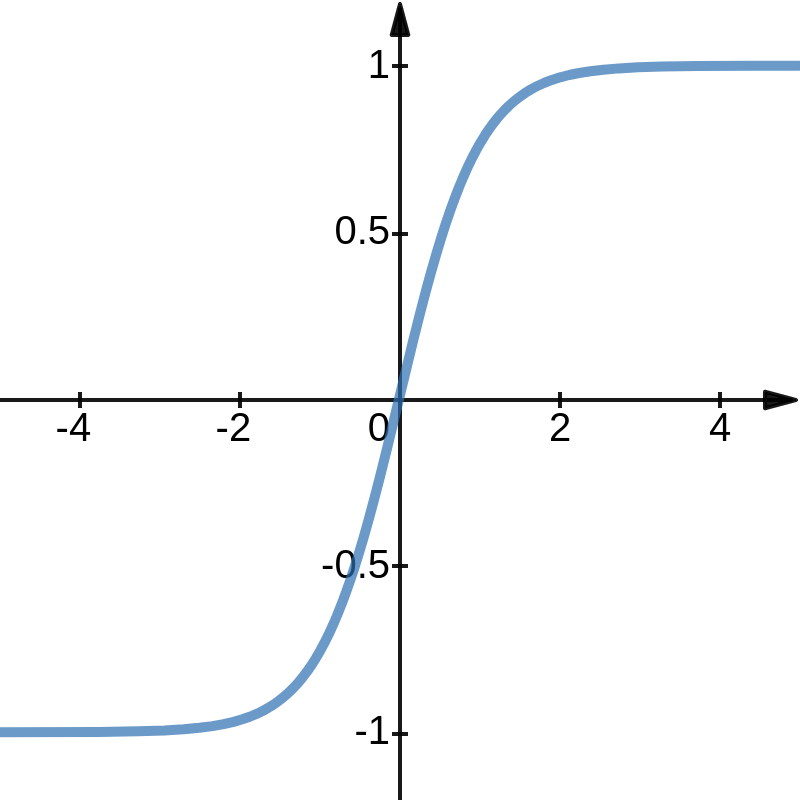
\includegraphics[width=.75\textwidth]{img/tanh_graph}
			\caption{Hiperbolinė tangento funkcija }
			\label{img:tanh_graph}
		\end{subfigure}%
		\begin{subfigure}[b]{.333\textwidth}
			\centering
			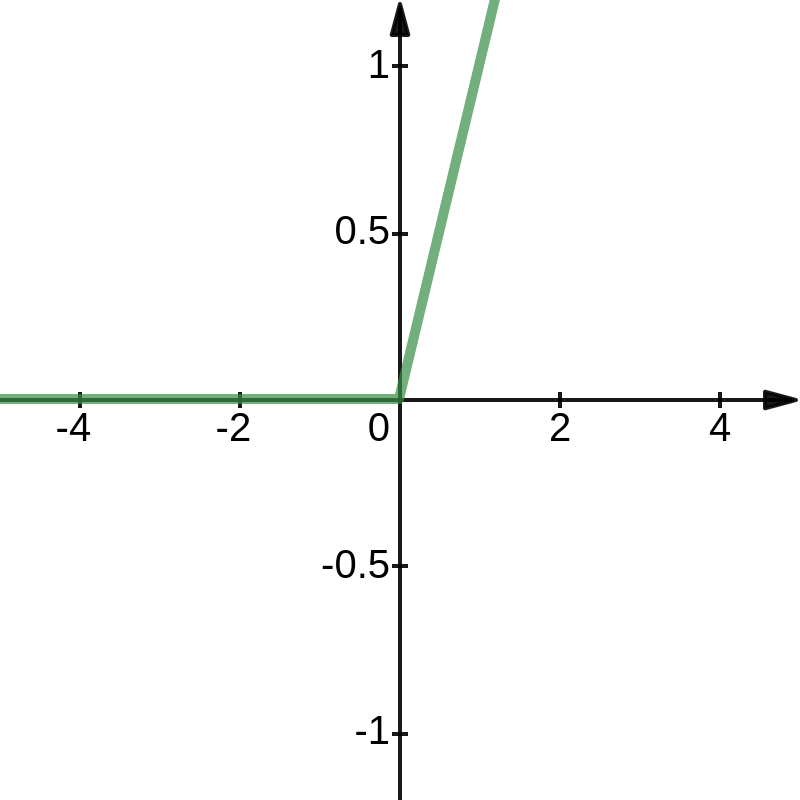
\includegraphics[width=.75\textwidth]{img/relu_graph}
			\caption{ReLU funkcija }
			\label{img:relu_graph}
		\end{subfigure}%
		\caption{Aktyvavimo funkcijų grafikai}
		\label{img:activation_graphs}
	\end{figure} 
	MLP yra dažnai naudojamas klasifikavimo uždaviniuose. Kai klasės yra diskrečios (pavyzdžiui, 6 skirtingos klasės su indeksais nuo 0 iki 5), išvesties sluoksnio individualios aktyvavimo funkcijos yra dažnai pakeičiamos viena bendra minkštojo maksimumo
	\footnote{Minkštojo maksimumo funkcija, dar žinoma kaip normalizuota eksponentės funkicija, yra funkcija, kuri realių skaičių vektoriu normalizuoja į tokio pat dydžio proporcingų tikimybių vektorių, kurio visų narių suma yra lygi 1. Matematinė išraiška: \(\sigma(\mathbf{z})_i = \frac{e^{z_i}}{\sum_{j=1}^K e^{z_i}} \textrm{ su visais } i = 1, \cdots, K \textrm{ ir } \mathbf{z} = (z_1, \cdots, z_K) \in \mathbb{R}^K \).}
	(\textit{angl. softmax}) funkcija, kuri padeda normalizuoti išvestis \cite{handson}.
}
\subsubsection{Konvoliuciniai neuroniniai tinklai}\label{subsubsec:cnn}
{
	Konvoluciniai neuroniniai tinklai (\textit{angl. convolutional neural networks}) (CNN) yra viena iš pagrindinių ML kategorijų atliekant: vaizdų atpažinimą, vaizdų klasifikavimą, objektų aptikimą, veidų atpažinimą ir pan. Tačiau CNN nėra limituoti tik vizualine įvestimi, juos taip pat galima pritaikyti dirbant su garsu ar natūraliam kalbos mokymui (\textit{angl. natural language processing}) \cite{cnn_online, handson}. Šiuolaikiniams CNN labai didelę įtaką turėjo regos smegenų žievės studijų įkvėptas neokognitronas\footnote{Neokognitronas -- Kunihiko Fukushima 1979 metais pristatytas hierarchinis daugiasluoksnis ANN. Buvo naudojamas ranka parašytų simbolių bei pasikartojančių ypatybių (\textit{angl. pattern}) atpažinimui.} \cite{fukushima1980neocognitron} bei 1998 metais pristatyta garsi \enquote{LeNet-5}\footnote{\enquote{LeNet-5} -- vienas pirmųjų CNN išplatinęs gilujį mokymasį, plačiai naudojamas ant čekių ranka urašytų skaičių atpažinimui.} architektūra \cite{lecun1998gradient}. \par
		
	Be pilnai sujungtų sluoksnių, CNN turi du papildomus architektūrinius komponentus:
	\begin{itemize}
		\item \textbf{Konvoliucinis sluoksnis} (\textit{angl. convolutional layers}).
		\item \textbf{Sutelkimo sluoksins} (\textit{angl. pooling layer}).
	\end{itemize}\par
	Toliau šiame punkte bus aprašomi minėtieji CNN architektūriniai komponentai.
}	
\subsubsubsection{Konvoliuciniai sluoksniai}\label{subsubsubsec:convolution_layer}
{
	Konvoliuciniai\footnote{Konvoliucija yra matematinė operacija, kuri per vieną funkciją pereina su kita ir išmatuoja taškinės daugybos integralą.} sluoksniai yra pats svarbiausias CNN architektūrinis komponentas. Pirmojo konvoliucinio sluoksnio neuronai nėra jungiami su kiekviena tiriamojo objekto įvestimi (pavyzdžiui, paveikslėlio pikseliu), bet tik su įvestimis kurios priklauso jų matymo laukui (\textit{angl. receptive field}). Tokiu pačiu principu, tolimesni konvoliuciniai sluoksniai yra jungiami su prieš tai buvusiais, kur gilesniame konvoliuciniame sluoksnyje esantis neuronas yra jungiamas tik su jo matymo laukui priklausančiais praeito sluoksnio neuronais. Pritaikius šią metodiką, žemesnio lygio sluoksniai yra atsakingi už paprastesnių požymių išskyrimą, o aukštesni už šių požymių apjungimą į sudėtingesnius.\par
	
	Sluoksnių ir matymo laukų dydžiai ne visada persidengia lygiai. Tokiais atvejais yra laikoma, kad visos matymo lauko reikšmės išeinančios iš tiriamojo sluoksnio ribų yra nuliai. Tai vadinama papildymu nuliais (\textit{angl. zero padding}).\par
	
	Jeigu prie didesnio sluoksnio yra jungiamas mažesnis, vienas iš būdų tą pasiekti yra darant didesnius tarpus tarp matymo laukų. Atstumas tarp dviejų matymo laukų yra vadinamas žingsniu (\textit{angl. stride}). Taip pat, verta paminėti, kad vertikalus ir horizontalus žingsniai neprivalo būti vienodo dydžio. \par
	
	Neuronų svoriai gali būti atvaizduojami mažais paveikslėliais, vadinamais filtrais arba konvoliucijų branduoliais (\textit{angl. convolution kernels}). Paveikslėlyje~\ref{img:cnn_filters} pavaizduoti du galimi filtrų pavyzdžiai, kairėje atvaizduotas filtras išryškina vertikalias linijas duotame paveikslėlyje, dešinėje -- horizontalias linijas išryškinantis filtras \cite{cnn_filters, handson}.
	\begin{figure}[H]
		\centering
		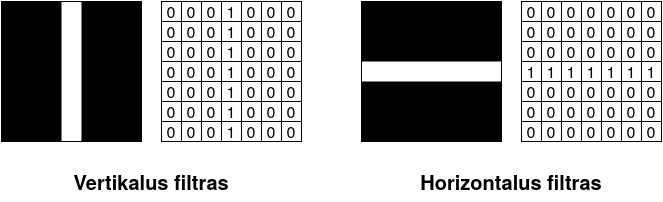
\includegraphics[scale=0.5]{img/cnn_filters}
		\caption{Konvoliucinių filtrų pavyzdžiai}
		\label{img:cnn_filters}
	\end{figure} 
	
	Konvoliucinio sluoksnio, kurio visi neuronai naudoja tą patį filtrą rezultatas yra vadinamas požymių žemėlapiu (\textit{angl. feature map}). Požymių žemėlapis išryškina paveikslėlio dalis, kurios yra labiausiai panašios į filtrą. Mokymosi metu CNN ieško naudingiausių filtrų bei jų kombinacijų duotai užduočiai atlikti. Viename konvoliuciniame sluoksnyje įvesčiai yra pritaikomi iškarto keli skirtingi filtrai, taip vienu metu aptinkami keli skirtingi požymiai. Kai yra naudojamas vienas požymių žemėlapis, visi neuronai naudoja vienodus parametrus, tačiau skirtingi žemėlapiai gali naudoti skirtingus svorius ir poslinkius. Viena iš šio principo naudų yra: visi neuronai naudoja tuos pačius filtrus, kai CNN išmoksta naują taisyklę vienoje įvesties dalyje, vėliau ją gali atpažinti bet kur įvestyje. \par
	
	Konvoliucinio sluoksnio neurono išvestį galima apskaičiuoti naudojantis formule~(\ref{eq:cnn}), kuri apskaičiuoja visų įvesčių svorių ir postūmių sumą.
	
	\begin{equation}\label{eq:cnn}
		z_{i, j, k} = b_k + \sum_{u=1}^{f_h} \sum_{v=1}^{f_w} \sum_{k'=1}^{f_n'} x_{i', j', k'} \cdot w_{u,v,k',k}
		\quad \textrm{kur} \
		\begin{cases}
			\begin{aligned}
				i' &= u \cdot s_h + f_h - 1 \\
				j' &= v \cdot s_w + f_w - 1 
			\end{aligned}
		\end{cases} 
	\end{equation}
	
	\begin{itemize}
		\item \(z_{i, j, k}\) konvoliucinio sluoksnio \(l\) eilutėje \(i\), stulpelyje \(j\), požymių žemėlapyje \(k\) esančio neurono išvestis.
		\item \(s_h\) ir \(s_w\) vertikalus ir horizontalus žingsniai.
		\item \(f_h\) ir \(f_w\) matymo lauko aukštis ir plotis.
		\item \(f_n'\) praeito sluoksnio \(l-1\) požymių žemėlapių skaičius.
		\item \(x_{i', j', k'}\) sluoksnyje \(l-1\), eilutėje \(i'\), stulpelyje \(j'\), požymių žemėlapyje \(k'\) esančio neurono išvestis.
		\item \(b_k\) sluoksnyje \(l\) esančiam požymių žemėlapiui \(k\) priskirtas postūmis.
		\item \(w_{u,v,k',k}\) ryšio svoris tarp neurono esančio požymių žemėlapyje \(k\) sluoksnyje \(l\) ir jo reliatyvios matymo laukui įvesties eilutėje \(u\), stulpelyje \(v\), požymių žemėlapyje \(k'\).
	\end{itemize}
}	
\subsubsubsection{Sutelkimo sluoksniai}
{
	Sutelkimo sluoksniai veikia labai panašiai kaip konvoliuciniai sluoksniai (žiūrėti papunktyje~\ref{subsubsubsec:convolution_layer}). Šio sluoksnio tikslas yra sumažinti (\textit{angl. subsample}) įvesties objektą, taip padidinant skaičiavimų greitį bei sumažinant reikalingos atminties kiekį ir parametrų skaičių. Paveikslėlio dydžio sumažinimas padeda ANN toleruoti mažus pakitimus (pavyzdžiui, pasukimus).\par
	
	Sluoksnyje esančių neuronų įvestys  yra sujungtos tik su matymo laukui priklausančia dalimi praeito sluoksnio išvesčių. Matymo laukas yra apibrėžiamas tais pačiais parametrais: dydžiu, žingsniu, užpildymo būdu. Sutelkimo, skirtingai nei konvoliucinio, sluoksnio neuronai neturi svorių. Vienintelė jų paskirtis yra surinkti ir sujungti įvestis pagal duotą funkciją (\textit{angl. aggregation function}) (pavyzdžiui, didžiausios (\textit{angl. max}) arba vidutinės (\textit{angl. mean}) reikšmės). Dažniausiai naudojamas sutelkimo sluoksnis yra sutelkimo imant maksimalią reikšmę sluoksnis (\textit{angl. max pooling layer}), kuris į tolimesnį sluoksnį perduoda tik kiekvieno matymo lauko didžiausias reikšmes \cite{handson}.\par
}

\subsubsection{Rekurentiniai neuroniniai tinklai}\label{subsubsec:rnn}
{
	Rekurentiniai neuroniniai tinklai (\textit{angl. recurrent neural networks}) yra ANN klasė, kur ryšiai tarp sujungimo taškų formuoja kryptinį grafą (gali jungtis su prieš tai buvusiais neuronais) ir skirtingai nei perceptronas (punktas~\ref{subsubsec:perceptron}), MLP (punktas~\ref{subsubsec:mlp}) ar CNN (punktas~\ref{subsubsec:cnn}) tai nėra tik į priekį einantis (\textit{angl. feedforward}) ANN. Ši architektūra leidžia RNN  prognozuoti (iki tam tikro lygio) ateities įvykius bei analizuoti laiko eilučių (\textit{angl. time series}) duomenis ar dirbti su nežinomo ilgio duomenų sekomis (\textit{angl. sequences}) \cite{handson}.
}
\subsubsubsection{Pasikartojantys neuronai}
{
	Neuronas, kuris gavęs įvestį apskaičiuoja išvestį ir perduoda naujai apskaičiuotą išvestį atgal sau kaip įvestį, yra vadinamas pasikartojančiu neuronu (\textit{angl. recurrent neuron}) (paveikslėlis~\ref{img:recurrent_neuron}). Paveikslėlyje~\ref{img:unrolled} pavaizduotas laike išvynioto (\textit{angl. unrolled through time}) RNN sudaryto tik iš vieno pasikartojančio neurono pavyzdys, kur kiekvieną laiko žingsnį (\textit{angl. time step}) \(t\) neuronas gauna įvestį \(x_{(t)}\) bei praeito žingsnio išvestį \(y_{(t-1)}\).
	
	\begin{figure}[H]
		\centering
		\begin{subfigure}[b]{.33\textwidth}
			\centering
			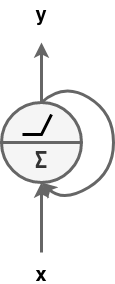
\includegraphics[scale=0.33]{img/recurrent_neuron}
			\caption{Pasikartojantis neuronas}
			\label{img:recurrent_neuron}
		\end{subfigure}%
		\begin{subfigure}[b]{.66\textwidth}
			\centering
			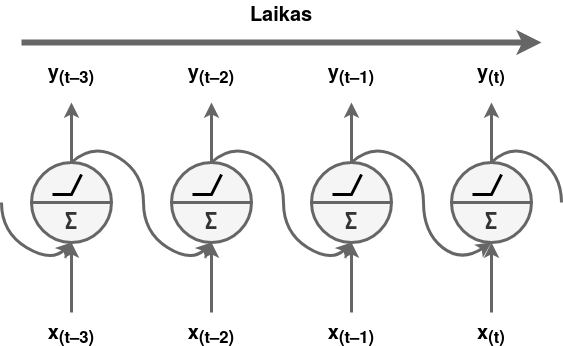
\includegraphics[scale=0.33]{img/unrolled}
			\caption{Laike išvyniotas pasikartojantis neuronas}
			\label{img:unrolled}
		\end{subfigure}
		\caption{Pasikartojančio neurono pavyzdžiai}
		\label{img:rnn_simple}
	\end{figure} 

	Sluoksnio iš pasikartojančių neuronų formavimas yra visiškai trivialus. Pagrindinis skirtumas, kad kiekviename laiko žingsnyje \(t\) kiekvienas neuronas gauna tiek visų naujų įvesčių vektorių \(\mathbf{x}_{(t)}\), tiek praeito laiko žingsnio išvesčių vektorių \(\mathbf{y}_{(t-1)}\). Be to, kiekvienas pasikartojantis neuronas turi du svorių rinkinius \(\mathbf{w}_x\) ir \(\mathbf{w}_y\): vienas įvestims \(\mathbf{x}_{(t)}\), kitas praeito laiko žingsnio išvestims \(\mathbf{y}_{(t-1)}\). Tada pasikartojančio neurono išvestį galima apskaičiuoti pasinaudojus formule \(y_{(t)} = \phi (\mathbf{x}_{(t)}^T \cdot \mathbf{w}_x + \mathbf{y}_{(t-1)}^T \cdot \mathbf{w}_y + b)\), kur \(\phi()\) yra aktyvavimo funkcija (pavyzdžiui, ReLU) (daugiau, punkte~\ref{subsubsec:mlp}), ir \(b\) yra postūmis \cite{handson}.\par
	
	Pasinaudojus formule~(\ref{eq:rnn_all_layer}) galima apskaičiuoti viso sluoksnio išvestį vienai mini-partijai\footnote{Mini-partija yra maža treniravimo duomenų dalis naudojama vienai mokymo iteracijai.} (\textit{angl. mini-batch}).
	
	\begin{equation}\label{eq:rnn_all_layer}
	\begin{split}
		\mathbf{Y}_{(t)} &= \phi (\mathbf{X}_{(t)} \cdot \mathbf{W}_x + \mathbf{Y}_{(t-1)} \cdot \mathbf{W}_y + \mathbf{b}) \\
		&= \phi (
		\begin{bmatrix}
			\mathbf{X}_{(t)} & \mathbf{Y}_{(t-1)}
		\end{bmatrix} 
		\cdot \mathbf{W}  + \mathbf{b}) \quad \textrm{kur} \ \mathbf{W} =
		\begin{bmatrix}
			\mathbf{W}_x \\
			\mathbf{W}_y
		\end{bmatrix}
	\end{split}
	\end{equation}

	\begin{itemize}
		\item \(\mathbf{Y}_{(t)}\) yra sluoksnio išvesties visai mini-partijai \(m \times n_{\textrm{neuronai}}\) matrica laiko žingsnyje \(t\), kur \(m\) yra mini-partijos dydis ir \(n_{\textrm{neuronai}}\) yra neuronų skaičius.
		\item \(\mathbf{X}_{(t)}\) yra visų įvesčių \(m \times n_{\textrm{įvestys}}\) matrica, kur \(n_{\textrm{įvestys}}\) yra įvesčių požymių skaičius.
		\item \(\mathbf{W}_x\) yra dabartinio laiko žingsnio įvesties ryšių svorių \(n_{\textrm{įvestys}} \times n_{\textrm{neuronai}}\) matrica.
		\item \(\mathbf{W}_y\) yra praeito laiko žingsnio išvesties ryšių svorių \(n_{\textrm{neuronai}} \times n_{\textrm{neuronai}}\) matrica.
		\item \(\mathbf{b}\) yra visų neuronų postūmių \(n_{\textrm{neuronai}}\) dydžio vektorius.
	\end{itemize}\par
	Jei skaičiuojama pirmo sluoksnio išvestis, buvusio laiko žingsnio išvestis (kadangi dar nėra įvykusi) dažniausiai laikoma nuliais.\par
	
	Pasikartojančio neurono išvestis galima išreikšti \(\mathbf{h}_{(t)}\) formule nuo laiko žingsnių \(t\), kuri yra priklausoma nuo visų iki tol buvusių įvesčių \(\mathbf{h}_{(t)} = f(\mathbf{h}_{(t-1)}, \mathbf{x}_{(t)})\), kur \(\mathbf{x}_{(t)}\) yra įvesčių vektorius žingsnyje \(t\). Todėl tai galima vadinti atmintimi. Neuroninio tinklo dalis sauganti tam tikrą būseną laike yra vadinama atminties ląstele (\textit{angl. memory cell}). Paveikslėlyje~\ref{img:rnn_simple} pavaizduota pasikartojanti ląstelė ar iš jų sudarytas sluoksnis yra laikomi paprastosiomis atminties ląstelėmis (\textit{angl. basic cell}).
}
\subsubsubsection{Ilgos trumpalaikės atminties modelis}\label{subsubsubsec:lstm}
{
	Ilgos trumpalaikės atminties modelio (\textit{angl. long short-teme memory}, LSTM) ląstelė \cite{hochreiter_schmidhuber_1997, sak2014long} gali būti naudojama panašiai kaip paprastosios atminties ląstelės, tačiau LSTM dažniausiai veiks geriau ir konverguos greičiau bei aptiks ilgalaikes priklausomybes duomenyse \cite{handson}.\par
	
	LSTM ląstelės (paveikslėlis~\ref{img:lstm}), skirtingai nei paprastoji atminties ląstelė turi du būsenos vektorius: \(\mathbf{h}_{(t)}\) trumpalaikei būsenai ir  \(\mathbf{c}_{(t)}\) -- ilgalaikei. Pagrindinė modelio idėja yra galimybė išmokti ką laikyti ilgalaikėje būsenoje ir žinoti kokius duomenis atmesti, ir kokius naudoti. Tai galima pamatyti paveikslėlyje~\ref{img:lstm} sekant rodyklę \(\mathbf{c}_{(t-1)}\), kurios pati pirma operacija ląstelėje yra vadinama pamiršimo vartais (\textit{angl. forget gate}). Išmetus dalį ilgalaikės būsenos informacijos ir pridėjus naujai gautą informaciją iš naujos įvesties, gautas vektorius \(\mathbf{c}_{(t)}\) yra tiesiai išvedamas kaip nauja ilgalaikė būsena.
	
	\begin{figure}[H]
		\centering
		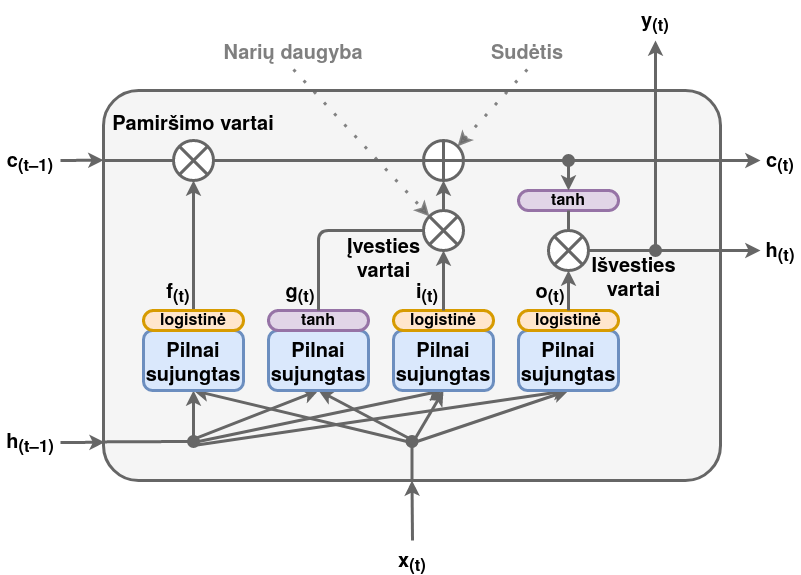
\includegraphics[scale=0.33]{img/lstm}
		\caption{Ilgos trumpalaikės atminties modelis}
		\label{img:lstm}
	\end{figure} 

	LSTM (paveikslėlis~\ref{img:lstm}) darbas prasideda su nauju įvesties vektorius \(\mathbf{x}_{(t)}\) ir praeita trumpalaike būsena \(\mathbf{h}_{(t-1)}\), kurie yra paduodami į keturis skirtingus pilnai sujungtus sluoksnius. Kiekvienas iš šių sluoksnių turi skirtinga paskirtį:
	
	\begin{itemize}
		\item Pagrindinis sluoksnis yr su išvesti \(\mathbf{g}_{(t)}\). Jo paskirtis yra išanalizuoti naujai paduoto įvesties vektoriaus \(\mathbf{x}_{(t)}\) ir praeitą trumpalaikių būsenų vektorių \(\mathbf{h}_{(t-1)}\).
		\item Kiti trys sluoksniai yra vadinami vartų valdikliai (\textit{angl. gate controllers}). Šie sluoksniai naudoja logistinę aktyvavimo funkciją, todėl jų išvestys yra \((0, 1)\) ribose. Jų visų išvestys yra paduodamos į atitinkamus vartus, kur yra atliekama narių daugyba\footnote{Apskaičiuojamas \enquote{Hadamardo daugyba} (\textit{angl. Hadamard product}). Hadamardo produktas tai yra matrica gaunama tarpusavyje sudauginus visus dviejų vienodo dydžio matricų elementus esančius tose pačiose vietose. Pavyzdžiui, 
			\(\begin{bmatrix} 1 & 2 & 3 \\ 4 & 5 & 6 \end{bmatrix} \circ
			\begin{bmatrix} 1 & 2 & 3 \\ 4 & 5 & 6 \end{bmatrix} =			
			\begin{bmatrix} 1 & 4 & 9 \\ 16 & 25 & 36 \end{bmatrix}\).
		}. Taip gauti \(0\) \enquote{uždaro} vartus ir \(1\) \enquote{atidaro}.
		\begin{itemize}
			\item \textbf{Pamiršimo vartai} -- valdomi vektoriau \(\mathbf{f}_{(t)}\) nustato kokia informacija turėtų būti pašalinama iš ilgalaikės būsenos.
			\item \textbf{Įvesties vartai} -- valdomi vektoriau \(\mathbf{i}_{(t)}\) nustato kokia dalis vektoriaus \(\mathbf{g}_{(t)}\) turėtų būti pridedama į ilgalaikę būseną.
			\item \textbf{Išvesties vartai} -- valdomi vektoriau \(\mathbf{o}_{(t)}\) nustato kokia dalis ilgalaikės būsenos turėtų būti išvesta šį laiko žingsnį į vektorius \(\mathbf{y}_{(t)}\) ir \(\mathbf{h}_{(t)}\).
		\end{itemize}
	\end{itemize}
}
\section{Metodologija}
{
	Šiame skyriuje analizuojama Sokoban aplinka ir jos pasirinkimai. Taip pat analizuojama RL biblioteka ir jos pasirinkimai. Analizuojami algoritmai ir strategijos.
}
\subsection{Sokoban žaidimas}
{
	Sokoban (iš japonų kalbos išvertus \enquote{sandėlio prižiūrėtojas}) yra 1981 metais Hiroyuki Imabayashi sukurtas tradicinis galvosūkis. Tai yra sudėtingas vieno žaidėjo žaidimas, kuriame tikslas yra vaikštant po labirintą priminantį \enquote{sandėlį} nustumti dėžes ant tikslo langelių. Kai visos dėžės yra ant tikslo langelių -- Sokoban laikomas išspręstu. Žaidimo sudėtingumas kyla iš jo apribojimų:
	\begin{enumerate}
		\item Žaidėjas gali judėti į visas keturias puses, tačiau negali pereiti kiaurai sienų ar dežių.
		\item Žaidėjas gali pastumti šalia jo esančią dėžę, jei stūmimo kryptimi už jos esantis laukelis yra tuščias.
		\item Žaidėjas negali pastumti daugiau nei vienos dėžės vienu metu.
		\item Žaidėjas negali traukti dėžių. 
	\end{enumerate}\par
	Sokoban neturi bendrojo sprendinio ar sprendimo būdo. Yra įrodyta, kad Sokoban yra NP-hard\footnote{NP-hard yra problemos, kurios yra tokio pat ar didesnio sudėtingumo, nei sudėtingiausios žinomos NP problemos. NP problemos yra klasė skaičiavimo problemų, kurios yra išsprendžiamos nedetriministiniu būdu polinominiame laike.} \cite{dor1999sokoban} ir PSPACE-complete\footnote{PSPACE-complete yra problemos, kurios gali būti išsprestos naudojantis polinominiu kiekiu atminties.} \cite{culberson1997sokoban} uždavinys.\par
	Papildomas sudėtingumo veiksnys yra neišsprendžiamų būsenų atliekant netinkamą veiksmą egzistavimas. Kadangi žaidėjui yra leidžiama tik stumti dėžes, situacijos, kur galvosūkis nebėra išsprendžiamas yra dažnos. Tokios žaidimo būsenos yra vadinamos aklavietėmis (\textit{angl. deadlock}) \cite{junghanns1998sokoban}. Aptikti Sokoban aklavietes yra taip pat ar net sudėtingiau nei išspręsti patį galvosūki, todėl tai irgi yra NP-hard uždavinys \cite{schaul2005evolving}.
}
\subsubsection{Aplinka}
Šiame punkte aprašoma aplinka ir jos pasirinkimo procesas.
\subsubsubsection{Aplinkos pasirinkimas}\label{subsubsubsec:environment_choice}
{
	Sokoban yra dažnas įvairių tyrimų objektas, todėl jam egzistuoja jau paruoštos aplinkos. Šias aplinkas galima panaudoti RL algoritmų apmokymams, taip pakartotinai nenaudojant resursų aplinkos implementacijai. \par
	Galimos viešai prieinamos atviro kodo Sokoban aplinkos:
	\begin{itemize}
		\item \textbf{XSokoban}\footnote{\url{http://www.cs.cornell.edu/andru/xsokoban.html}} \cite{myers1995xsokoban} -- moksliniuose darbuose dažna Sokoban žaidimo implementacija. XSokoban yra sudarytas iš 90 sudėtingų galvosūkių ir leidžia varžytis su kitais geriausiais Sokoban žaidėjais. Tačiau ši platforma veikia tik su Unix (Linux) sistemomis ir paskutinį kartą buvo atnaujinta tik 1997 metų liepą.
		\item \textbf{Gym-Sokoban} \cite{SchraderSokoban2018} -- ant OpenAI Gym \cite{openaiGym} karkaso pastatyta Sokoban aplinka, kurios implementacija yra paremta \enquote{DeepMind\footnote{\enquote{Google} priklausanti dirbtinio intelekto tyrimų kompanija, garsi savo \enquote{AlphaGo} programa, 2016 mettais laimėjusia prieš \enquote{Go} žaidimo pasaulio čempijoną Lee Sedol.}} pateiktu taisyklių rinkiniu aplinkoms \cite{NIPS2017_7152}. Taip pat ši aplinka generuoja kambarius atsitiktinai, kas leidžia mokyti DNN be perpildymo (\textit{angl. overfitting}).
	\end{itemize}

	Darbui atlikti buvo pasirinkta naudoti Gym-Sokoban aplinką, dėl jos modernumo ir implementacijos paremtos OpenAI Gym karkasu, kuris yra tapęs RL aplinkų standartu. Taip pat, kadangi darbo metu bus naudojami modernūs DNN paremti RL algoritmai -- atsitiktinis kambarių generavimas yra didelis pranašumas.
}
\subsubsubsection{OpenAI Gym aplinkos}\label{subsubsubsec:gym}
{
	Gym yra, \enquote{OpenAI\footnote{Dirbtinio intelekto sprendimų vystymo ir pritaikymo kompanija. \url{https://openai.com/about/}}} kompanijos kuriamas, RL algoritmų kūrimo ir palyginimo įrankių rinkinys. Šie įrankiai nedaro jokių prielaidų apie agento struktūrą bei yra pritaikomi su daugeliu skaičiavimo bibliotekų \cite{openaiGym}.\par
	
	\code{gym}\footnote{\url{https://github.com/openai/gym}} yra atviro kodo Python biblioteka. Centrinis bibliotekos interfeisas yra unifikuota aplinkos sąsaja \code{Env}, kurios pagrindiniai metodai yra:
	\begin{itemize}
		\item \code{\textbf{reset(self) -> observation}} -- atstato aplinkos parametrus į pradines reikšmes, bei grąžina naują jos būseną.
		\item \code{\textbf{step(self, action) -> observation, reward, done, info}} -- aplinkos laiko žingsnio metodas, kuriam paduodamas pasirinktas veiksmas ir grąžinama: nauja aplinkos būsena, atlikto veiksmo atlygis, \code{bool} tipo reikšmė, nurodanti ar aplinka buvo užbaigta, bei papildoma (paprastai nenaudotina algoritmo mokymui) informacija apie aplinką .
		\item \code{\textbf{render(self, mode='human')}} -- atvaizduojamas vienas aplinkos kadras. Numatytuoju būdu, metodas turėtų atlikti tai žmogui lengvai suprantamu būdu.
	\end{itemize}\par

	\code{Wrapper} yra dekoratoriaus dizaino modelio implementacija, leidžianti dinamiškai papildyti naujomis ar išplėsti esamas \code{Env} aplinkos objekto funkcijas.
}
\subsubsubsection{Gym-Sokoban}\label{subsubsubsec:gym-sokoban}
{
	\code{gym-sokoban} yra Python biblioteka, kuri leidžia sukurti OpenAI Gym (papunktis~\ref{subsubsubsec:gym}) paremtą Sokoban žaidimo aplinką pritaikytą RL algoritmų apmokymams. Pagrindinis bibliotekos objektas yra, \code{gym.Env} interfeiso implementacija, \code{SokobanEnv} -- Sokoban žaidimo aplinka.\par
	
	\code{gym-sokoban} turi penkias skirtingas Sokoban žaidimo variacijas (pavyzdžiui, variacija, kur žaidėjas gali stumti ir traukti dėžes), tačiau darbas bus atliekamas ir toliau aprašoma tik standartinė, artimiausia tradiciniam Sokoban žaidimui, variacija.\par
	
	Kambariai yra sudaromi iš penkių tipų elementų: sienų, grindų, dėžių, tikslų ir žaidėjo, tačiau kai kurie iš jų gali persidengti ir turi kelias skirtingas būsenas. Visos šios kambario elementų ir būsenų variacijos yra reprezentuojamos žaidime atskiru \(16 \times 16\) pikselių paveikslėliu (lentelė~\ref{tab:sokoban_tiles}). 
	
	\begin{table}[H]
		\caption{Sokoban žaidimo aplinkos elementų būsenos ir jų grafinės reprezentacijos}
		\label{tab:sokoban_tiles}
		\centering
		\begin{tabular}{llc}
			\toprule
			\multicolumn{1}{c}{\textbf{Tipas}} &
			\multicolumn{1}{c}{\textbf{Būsena}} &
			\textbf{\begin{tabular}[c]{@{}c@{}}Grafinė\\ reprezentacija\end{tabular}} \\ 
			\midrule
			
			Siena & Statinė & 
\includegraphics[scale=.6]{img/sokoban/tiles/wall} \\ 
			\rowcolor[HTML]{EFEFEF} 
			Grindys & Tuščios & 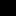
\includegraphics[scale=.6]{img/sokoban/tiles/floor} \\ 
			Tikslas & Tuščias & 
\includegraphics[scale=.6]{img/sokoban/tiles/box_target} \\ 
			\rowcolor[HTML]{EFEFEF} 
			Dėžė & Ne ant tikslo & 
\includegraphics[scale=.6]{img/sokoban/tiles/box} \\ 
			Dėžė & Ant tikslo & 
\includegraphics[scale=.6]{img/sokoban/tiles/box_on_target} \\ 
			\rowcolor[HTML]{EFEFEF}  
			Žaidėjas & Ne ant tikslo & 
\includegraphics[scale=.6]{img/sokoban/tiles/player} \\
			Žaidėjas & Ant tikslo & 
\includegraphics[scale=.6]{img/sokoban/tiles/player_on_target} \\ 
			
			\bottomrule
		\end{tabular}
	\end{table}
	Standartinė aplinka priima devynis skirtingus veiksmus: nieko neveikimo veiksmas (\(0\)), po veiksmą dėžės pastūmimams (\(1-5\)) ir po veiksmą paėjimams (\(6-7\)) į visas keturias puses (aukštyn, žemyn, kairėn ir dešinėn). Judėjimo veiksmai yra atliekami tik tuo atveju, jei laukelis nurodyta kryptimi yra tuščias; pastūmimo veiksmai turi dvi variacijas, jei laukelis nurodytai kryptimi tuščias -- paeinama į jį, jei tas laukelis yra dėžė ir už jos tuščia -- pastumiama dėžė.\par
	
	Visos RL aplinkos turi duoti agentui atlygį už atliktą veiksmą (poskyris~\ref{subsec:RL}). Gym-Sokoban aplinka galimai duoda vieną ar kelis iš keturių atlygių:
	\begin{itemize}
		\item \(\mathbf{+10,0}\) -- už visų dėžių buvimą ant tikslo laukelių.
		\item \(\mathbf{+1,0}\) -- už dėžės užstūmimą ant tikslo.
		\item \(\mathbf{–1,0}\) -- už dėžės nustūmimą nuo tikslo.
		\item \(\mathbf{–0,1}\) -- už atliktą veiksmą.
	\end{itemize}
	
	Aplinka bibliotekoje yra apibrėžiama \code{SokobanEnv} klase, kuri yra atsakinga už kambarių generavimą ir veiksmų interpretavimą, bei atlygio už atliktą veiksmą apskaičiavimą. Generuojamų kambarių savybės (paveikslėlis~\ref{img:sokoban_examples}) yra nurodomos klasės konstruktoriumi, kurios leidžia modifikuoti parametrus:
	\begin{itemize}
		\item \textbf{Kambario dydį} (\code{tuple(int, int)})-- generuojamų kambarių aukštis ir plotįis.
		\item \textbf{Dėžių kambaryje skaičių} (\code{int})-- kiek dėžių ir tikslo laukelių bus sugeneruojame per kambarį.
		\item \textbf{Maksimalų žingsnių skaičių} (\code{int})-- jei žaidėjas neužbaigia kambario per nurodytą žingsnių skaičių, aplinka yra užbaigiama.
	\end{itemize}

	Agentui aplinkos būsenos yra duodamos trimačiu \((16 n_{\textrm{aukštis}}) \times (16 n_{\textrm{plotis}}) \times n_{\textrm{kanalų skaičius}} \) dydžio masyvu, kur \(\textrm{aukštis}\) ir \(\textrm{plotis}\) yra kambario dydis laukeliais (dauginamas iš \(16\) dėl pikselių skaičiaus per laukelį), \(n_{\textrm{kanalų skaičius}} = 3\) yra RGB spalvų kanalų skaičius, o reikšmės yra sveiki skaičiai \([0, 255]\) ribose.
	
	\begin{figure}[H]
		\centering
		\begin{subfigure}[b]{.2\textwidth}
			\centering
			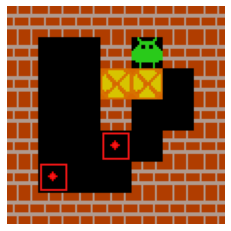
\includegraphics[scale=0.4]{img/sokoban/rooms/4}
			\captionsetup{justification=centering}
			\caption{2 dėžės,\\ \(7 \times 7\) kambarys}
			\label{img:room_1}
		\end{subfigure}%
		\begin{subfigure}[b]{.2\textwidth}
			\centering
			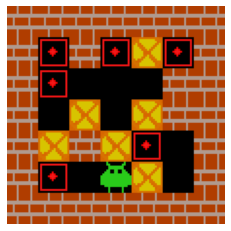
\includegraphics[scale=0.4]{img/sokoban/rooms/5}
			\captionsetup{justification=centering}
			\caption{6 dėžės,\\ \(7 \times 7\) kambarys}
			\label{img:room_2}
		\end{subfigure}%
		\begin{subfigure}[b]{.2\textwidth}
			\centering
			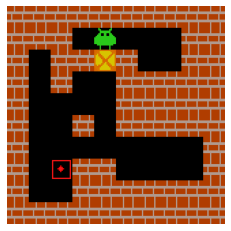
\includegraphics[scale=0.4]{img/sokoban/rooms/3}
			\captionsetup{justification=centering}
			\caption{1 dėžė,\\ \(10 \times 10\) kambarys}
			\label{img:room_3}
		\end{subfigure}%
		\begin{subfigure}[b]{.2\textwidth}
			\centering
			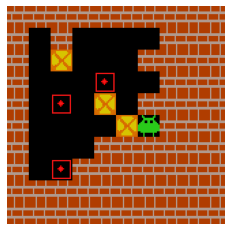
\includegraphics[scale=0.4]{img/sokoban/rooms/1}
			\captionsetup{justification=centering}
			\caption{3 dėžės,\\ \(10 \times 10\) kambarys}
			\label{img:room_4}
		\end{subfigure}%
		\begin{subfigure}[b]{.2\textwidth}
			\centering
			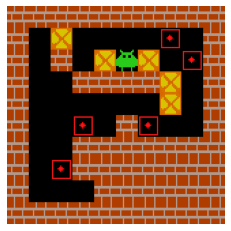
\includegraphics[scale=0.4]{img/sokoban/rooms/2}
			\captionsetup{justification=centering}
			\caption{5 dėžės,\\ \(10 \times 10\) kambarys}
			\label{img:room_5}
		\end{subfigure}%
		\caption{Sokoban žaidimo aplinkos skirtingo dydžio ir dėžių skaičiaus pavyzdžiai}
		\label{img:sokoban_examples}
	\end{figure} 
}
\subsection{Skatinamojo mokymosi biblioteka}
Šiame poskyryje aprašoma skatinamojo mokymosi biblioteka ir jos pasirinkimo procesas.
\subsection{Skatinamo mokymosi bibliotekos pasirinkimas}
{
	ML ir RL esant didelio susidomėjimo ir nuolatinių tyrimų objektais, natūraliai, moksliniuose darbuose pasiūlytos algoritmų implementacijos atsiranda ir cirkuliuoja viešai prieinamoje internetinėje erdvėje. Iš šių algoritmų yra formuojami rinkiniai ir RL bibliotekos. Tačiau bibliotekos turi savo naudojamus karkasus ir dažnai standartizuotą jų panaudojimo būdą. Renkantis RL biblioteką yra svarbu atsižvelgti į įvairius faktorius:  bibliotekos algoritmų rinkinį ir jų modernumą, kuriamo modelio aplinką ir jo karkasą, algoritmų naudojamas skaičiavimų bibliotekas, bibliotekos apibrėžtų objektų išplečiamumą ar naujų implementacijos sudėtingumą, pačios bibliotekos naudojimo sudėtingumą, programavimo kalbą ir panašiai \cite{simonini_2019}.\par
	
	Kelios dažniausiai naudojamos RL bibliotekos yra:
	\begin{itemize}
		\item \textbf{TF-Agents} \cite{TFAgents} -- šiame sąraše naujausia RL biblioteka, su daug žadančia moduline struktūra bei aukštos kokybės algoritmų implementacija. Ši biblioteka yra neoficialiai, kuriama pačio TensorFlow. Tačiau, kadangi tai yra jaunas produktas, biblioteka turi trūkumų: neturi dokumentacijos, dėl to, panaudojimas ar savo aplinkos pritaikymas nėra visiškai trivialus. Pilnas TensorBoard\footnote{TensorFlow vizualizacijos įrankis. \url{https://github.com/tensorflow/tensorboard}} palaikymas.
		
		\item \textbf{KerasRL} \cite{plappert2016kerasrl} -- RL biblioteka paremta Keras\footnote{Aukšto lygio ANN API parašyta su Python, kurios pagrindinis tikslas yra sudaryti sąlygas greitam eksperimentavimui.}. Nors kodas yra gerai komentuotas ir naudojamas geras agento, strategijos ir atminties atskyrimas, biblioteka nebuvo atnaujinta nuo 2019 metų. Bibliotekos algoritmų rinkinys yra limituotas, nors rinkinyje esami algoritmai yra modernus. Naujos aplinkos pridėjimas nėra galimas, nebent aplinka yra paremta OpenAI Gym (papunktis~\ref{subsubsubsec:gym}).
		
		\item \textbf{Tensorforce} \cite{tensorforce} -- modalių komponentų pagrindų sukurta, TensorFlow paremta RL biblioteka. Bibliotekos algoritmų rinkinyje yra didžioji dalis modernių RL algoritmų, tačiau pritaikymas nėra elementarus, dėl nepilnos algoritmų dokumentacijos. Biblioteka yra nuolatos naujinama bei yra lengvai modifikuojama, tačiau kodas beveik neturi komentarų. Pilnas TensorBoard palaikymas.
		
		\item \textbf{OpenAI Baselines} \cite{baselines} -- aukštos kokybes modernių RL algoritmų implementacijų rinkinys. Tačiau dokumentacijos dėl dokumentacijos trūkumo, naudotis biblioteka, suprasti kodą ar pritaikyti savo aplinkai yra sudėtinga. Nėra palaikomas TensorBoard.
		
		\item \textbf{Stable Baselines} \cite{stable-baselines} -- gerokai pagerinta OpenAI Baselines atšaka, su unifikuota algoritmų struktūra bei plačia dokumentacija. OpenAI Baselines modernių algoritmų implementacijos yra praplėstos naujais algoritmais, taip pat, originalus kodas yra papildytas komentarais ir TensorBoard palaikymu. Lengva pradėti naudotis, tačiau aplinkos yra limituotos OpenAI Gym (papunktis~\ref{subsubsubsec:gym}) karkaso.
	\end{itemize}\par

	Darbo metu buvo nuspręsta naudotis Stable Baselines, dėl kelių pagrindinių priežasčių. Kadangi Sokoban žaidimo pasirinkta aplinka (papunktis~\ref{subsubsubsec:environment_choice}) yra paremta OpenAI Gym karkasu, tai nėra laikoma aplinkos trūkumu. Pagrindinis rodiklis buvo modernių algoritmų implementacijų rinkinys, kuo KerasRL nepasižymi ir buvo atmestas. Kitas rodiklis buvo dokumentacija ir jos kokybė, ko TF-Agents ir OpenAI Baselines bibliotekos neturi, o Tensorfoce turi tačiau algoritmų dokumentacijos yra limituotos. Dar vienas rodiklis buvo, TensorBoard palaikymas, dėl galimybės stebėti algoritmo mokymą realiu laiku, ko neturi OpenAI Gym. Dėl šių priežasčių, pasirinkimo sąrašas buvo susiaurintas iki dviejų: Stable Baselines ir Tensorforce. Nors abu pasirinkimai yra geri, buvo nuspręsta naudotis Stable Baselines dėl paprastesnės naudojimo metodikos.
}
\subsubsection{Stable Baselines skatinamojo mokymosi biblioteka}\label{subsubsec:stable-baselines}
{
	Stable Baselines \cite{stable-baselines} yra rinkinys pagerintų RL algoritmų paremtų OpenAI Baselines \cite{baselines} implementacijomis. Ši RL biblioteka sudaryta iš plataus modernių algoritmų pasirinkimo. Tačiau, priklausomai nuo aplinkos veiksmų ir būsenų tipų, ne visi algoritmai gali jai būti pritaikyti (lentelė~\ref{tab:stable-baselines_algorithms}). Taip pat, biblioteka yra padalinta į dvi dalis: algoritmus naudojančius OpenMPI\footnote{Žinučių perdavimo sąsajos biblioteka.} jų lygiagretinimui, ir nenaudojančius OpenMPI.
	\begin{table}[H]
		\centering
		\caption{Stable Baselines algoritmai ir jų priimami aplinkų veiksmų ir būsenų tipai}
		\label{tab:stable-baselines_algorithms}
		\begin{tabular}{p{2cm}P{1cm}P{1cm}P{1cm}P{1cm}P{1cm}P{1cm}P{1cm}P{1cm}P{1.5cm}}
			\toprule
			\multicolumn{1}{P{2.25cm}}{} &
			\multicolumn{4}{p{5.5cm}}{\begin{tabular}{P{8.5cm}} \textbf{Galimi veiksmų tipai}\end{tabular}} &
			\multicolumn{4}{P{5.5cm}}{\begin{tabular}{P{8.5cm}} \textbf{Galimi būsenų tipai}\end{tabular}} \\
			\textbf{Algoritmai} &
			\rotatebox[origin=l]{45}{\begin{tabular}{p{3cm}} \textbf{Discrete} \\ \hline \end{tabular}} &
			\rotatebox[origin=l]{45}{\begin{tabular}{p{3cm}} \textbf{Box} \\ \hline \end{tabular}} &
			\rotatebox[origin=l]{45}{\begin{tabular}{p{3cm}} \textbf{MultiDiscrete} \\ \hline \end{tabular}} &
			\rotatebox[origin=l]{45}{\begin{tabular}{p{3cm}} \textbf{MultiBinary} \\ \hline \end{tabular}} &
			\rotatebox[origin=l]{45}{\begin{tabular}{p{3cm}} \textbf{Discrete} \\ \hline \end{tabular}} &
			\rotatebox[origin=l]{45}{\begin{tabular}{p{3cm}} \textbf{Box} \\ \hline \end{tabular}} &
			\rotatebox[origin=l]{45}{\begin{tabular}{p{3cm}} \textbf{MultiDiscrete} \\ \hline \end{tabular}} &
			\rotatebox[origin=l]{45}{\begin{tabular}{p{3cm}} \textbf{MultiBinary} \\ \hline \end{tabular}} & 
			\textbf{MPI} \\
			\midrule
			
			\textbf{A2C} & \cmark & \cmark & \cmark & \cmark & \cmark & \cmark & \cmark & \cmark & \xmark \\
			\rowcolor[HTML]{EFEFEF} 
			\textbf{ACER} & \cmark & \xmark & \xmark & \xmark & \cmark & \cmark & \cmark & \cmark & \xmark \\
			\textbf{ACKTR} & \cmark & \cmark & \xmark & \xmark & \cmark & \cmark & \cmark & \cmark & \xmark \\
			\rowcolor[HTML]{EFEFEF} 
			\textbf{DDPG} & \xmark & \cmark & \xmark & \xmark & \cmark & \cmark & \cmark & \cmark & \cmark \\
			\textbf{DQN} & \cmark & \xmark & \xmark & \xmark & \cmark & \cmark & \cmark & \cmark & \xmark \\
			\rowcolor[HTML]{EFEFEF} 
			\textbf{GAIL} & \cmark &  \cmark & \xmark & \xmark & \cmark & \cmark & \cmark & \cmark & \cmark \\
			\textbf{PPO1} & \cmark & \cmark & \cmark & \cmark & \cmark & \cmark & \cmark & \cmark & \cmark \\
			\rowcolor[HTML]{EFEFEF} 
			\textbf{PPO2} & \cmark & \cmark & \cmark & \cmark & \cmark & \cmark & \cmark & \cmark & \xmark \\
			\textbf{SAC} & \xmark & \cmark & \xmark & \xmark & \cmark & \cmark & \cmark & \cmark & \xmark \\
			\rowcolor[HTML]{EFEFEF} 
			\textbf{TD3} & \xmark & \cmark & \xmark & \xmark & \cmark & \cmark & \cmark & \cmark & \xmark \\
			\textbf{TRPO} & \cmark & \cmark & \cmark & \cmark & \cmark & \cmark & \cmark & \cmark & \cmark \\
			
			\bottomrule
		\end{tabular}
	\end{table}
	Kadangi bakalauro darbui pasirinktos aplinkos (papunktis~\ref{subsubsubsec:gym-sokoban}) veiksmų tipas yra \code{Discrete}\footnote{OpenAI Gym diskrečių sveikų skaičių masyvo tipas, kur sukurtas \(n\) dydžio kintamasis susideda iš \((0, 1, \cdots, n-1)\) skaitmenų.}, algoritmai, kurie nepalaiko šio tipo, nėra pritaikomi. Taip pat, autorių siūlymu, dėl esamos programinės klaidos, algoritmai naudojantys OpenMPI, darbo metu nebus naudojami. Atmetus algoritmus pagal šiuos du kriterijus lieka tik penki:
	\begin{itemize}
		\item \textbf{A2C} \cite{a3c} -- sinchroninis, determinuotas pranašumo aktoriaus-kritiko RL algoritmas, naudojantis kelis darbuotojus, pakartojimo buferio išvengimui.
		\item \textbf{ACER} \cite{acer} -- aktoriaus-kritiko RL algoritmas, sujungia keletą RL algoritmų idėjų: naudojasi keliais darbuotojais (kaip A2C), implementuoja patirties pakartojimo buferį (kaip DQN), naudoja atsekimo funkciją (\textit{angl. Retrace}) Q-vertės įvertinimui, svarbos atrinkimui ir pasitikėjimo sričiai.
		\item \textbf{ACKTR} \cite{acktr} -- aktoriaus-kritiko RL algoritmas, naudojanti Kroneckerio (\textit{angl. Kronceker-factored}) apskaičiuotą apytikslį kreivumą pasitikėjimo srities optimizavimui.
		\item \textbf{DQN} \cite{dqn} -- RL algoritmas derinantis Q-mokymąsi su DNN, leidžiančiais RL dirbti sudėtingose, didelėse erdvėse.
		\item \textbf{PPO2} \cite{ppo} -- aktoriaus-kritiko RL algoritmas sujungia A2C (turinčio kelis darbuotojus) ir TRPO (algoritmas naudoja pasitikėjimo sritį aktoriaus gerinimui).
	\end{itemize}
}
\subsubsubsection{Stable Baselines Karkasas}\label{subsubsubsec:stable-baselines_framework}
{
	Stable Baselines turi standartizuotą algoritmų naudojimo būdą. Pagrindiniai modelių metodai:
	\begin{itemize}
		\item \textbf{\textit{Konstruktorius}} -- konstruktoriui yra paduodami algoritmo ir strategijos hiper-parametrai bei aplinka. Grąžinamas paruoštas mokymui modelis.
		
		\item \textbf{\code{learn(total\_timesteps, \(\cdots\))}} -- grąžina nurodytą laiko žingsnių kiekį apmokytą modelį. Taip pat, galima nurodyti ankstesnio atšaukimo ar kitas taisykles bei duomenų registravimo vardą ar dažnumą.
		
		\item  \textbf{\code{save(save\_path, \(\cdots\))}} -- išsaugo modelį į nurodyto adreso failą.
		
		\item  \textbf{\code{load(load\_path, env=None, \(\cdots\))}} -- užkrauna modelį iš failo arba iš \code{Dictionary} tipo objekto. Jei naudojama tik veiksmų progrnozėms, aplinkos nurodyti nereikia, tačiau jei bus mokoma toliau, reikia nurodyti aplinką.
		
		\item \textbf{\code{predict(observation, \(\cdots\))}} -- padavus aplinkos būseną, modelis atlieką prognozės apskaičiavimą ir grąžina geriausią veiksmą. Galima papildomai nurodyti ar naudoti determinuotą principą ar ne.
	\end{itemize}
	
	Stable Baselines turi būdą sudėti kelias aplinkas į vieną vektorių. Šie aplinkų vektoriai yra pritaikomi daugeliui bibliotekos algoritmų ir leidžia vienu metu treniruoti modelį su keliomis aplinkomis. Jei naudojamos vektorinės aplinkos, vietoje būsenos ir veiksmų, modeliui yra paduodami aplinkų būsenų ir veiksmų vektoriai. Karkase yra apibrėžtos dviejų rūšių vektorinės aplinkos:
	\begin{itemize}
		\item \textbf{\code{DummyVecEnv}} -- paprastas vektorinis adapteris, kviečiantis visas aplinkas iš eilės.
		\item \textbf{\code{SubprocVecEnv}} -- daugiaprocesis vektorinis adapteris, kur kiekviena aplinka turi savo procesą ir kviečiant aplinkos funkciją, kadangi visos aplinkos veikia lygiagrečiai, atlieką skaičiavimus vienu metu.
	\end{itemize}

	Mokymo metu galima modeliui paduoti iškviečiamas (\textit{angl. callback}) funkcijas, kurios priklausomai nuo funkcijos gali būti iškviečiamos nurodytą mokymo proceso etapą. Naudojant šias funkcijas, galima pasiekti vidines modelio būsenas bei nutraukti mokymo procesą anksčiau. Iškviečiamų funkcijų rašymui yra apibrėžtas \code{BaseCallback} interfeisas. Taip pat, yra kelios funkcijų implementacijos, kurias galima panaudoti skirtingų užduočių atlikimui: periodiniam saugojimui, modelio tarpiniam vertinimui, išankstinio modelio mokymo stabdymui pasiekus nurodytą slenkstinį atlygį ir panašiai.
	
}
\subsubsection{Stable Baselines strategijos}\label{subsubsec:policies}
{
	Stable Baselines turi rinkinį numatytųjų strategijų, paremtų ANN (poskyris~\ref{subsec:neuro}). Pagrindinės dvi kategorijos yra MLP (punktas~\ref{subsubsec:mlp}) ir CNN (punktas~\ref{subsubsec:cnn}). Tačiau, kadangi bakalauro darbui pasirinktos aplinkos būsenos yra pateikiamos kadro pikselių masyvais (papunktis~\ref{subsubsubsec:gym-sokoban}), mokymo metu buvo pasirinktos tik CNN strategijos.\par
	
	Stable Baselines turi trijų rūšių CNN paremtas strategijas: paprastą CNN, LSTM (papunktis~\ref{subsubsubsec:lstm}) su CNN požymių išskyrimu, normalizuotą LSTM su CNN požymių išskyrimu. Toliau, šiame punkte bus aprašomos šios trys strategijos.
}
\subsubsubsection{CnnPolicy strategijos aprašymas}\label{subsubsubsec:cnnpolicy}
{	
	\code{CnnPolicy} yra viena iš Stable Baselines bibliotekos numatytųjų strategijų. Ši strategija naudoja CNN (punktas~\ref{subsubsec:cnn}) požymių išskyrimui ir dėl to yra geriausiai pritaikoma aplinkoms, kurių būsenos yra paduodamos aplinkos kadrų pikselių masyvais.\par
	
	Strategijos DNN architektūra yra sudaryta iš trijų konvoliucinių sluoksnių (papunktis~\ref{subsubsubsec:convolution_layer}) ir vieno paslėpto pilnai sujungto sluoksnio (lentelė~\ref{tab:cnnpolicy}). Visi šie sluoksniai naudoja ReLU aktyvavimo funkcijas (punktas~\ref{subsubsec:mlp}), tačiau išvesties aktyvavimo funkcija priklauso nuo aplinkos veiksmo tipo (lentelė~\ref{tab:stable-baselines_algorithms}). Bakalauro darbui parinkta Sokoban aplinka (papunktis~\ref{subsubsubsec:gym-sokoban}) naudoja \code{Discrete} tipo veiksmus, tokiu atveju išvesčiai naudojama bendra minkštojo maksimumo aktyvavimo funkcija  (punktas~\ref{subsubsec:mlp}).\par
	
	\begin{table}[H]
		\centering
		\caption{\code{CnnPolicy} strategijos ANN architektūrą sudarančių sluoksnių parametrai}
		\label{tab:cnnpolicy}
		\begin{tabular}{llcccc}
			\toprule
			\multicolumn{1}{c}{\textbf{Pavadinimas}} & \multicolumn{1}{c}{\textbf{\begin{tabular}[c]{@{}c@{}}Sluoksnio\\ tipas\end{tabular}}} & \textbf{\begin{tabular}[c]{@{}c@{}}FIltrų\\ skaičius\end{tabular}} & \textbf{\begin{tabular}[c]{@{}c@{}}Filtrų\\ dydis\end{tabular}} & \textbf{Žingsnis} & \textbf{\begin{tabular}[c]{@{}c@{}}Neuronų\\ skaičius\end{tabular}} \\
			\midrule
			c1 & Konvoliucinis & 32 & 8 & 4 & -- \\
			\rowcolor[HTML]{EFEFEF} 
			c2 & Konvoliucinis & 64 & 4 & 2 & -- \\
			c3 & Konvoliucinis & 64 & 3 & 1 & -- \\
			\rowcolor[HTML]{EFEFEF} 
			fc1 & Pilnai sujungtas & -- & -- & -- & 512 \\
			\bottomrule
		\end{tabular}
	\end{table}
}
\subsubsubsection{CnnLstmPolicy strategijos aprašymas}\label{subsubsubsec:cnnlstmpolicy}
{
	\code{CnnLstmPolicy} strategija yra labai panaši \code{CnnPolicy} strategijai (papunktis~\ref{subsubsubsec:cnnpolicy}). Tačiau šios strategijos architektūra yra RNN (punktas~\ref{subsubsec:rnn}) ir tie patys \code{CnnPolicy} sluoksniai yra naudojami LSTM atminties ląstelės (papunktis~\ref{subsubsubsec:lstm}) įvesčiai. LSTM ląstelė yra standartinė, su keturiais pilnai sujungtais sluoksniais, kurių kiekvieno dydis yra \(256\) neuronai. Išvestis yra valdoma identiškai \code{CnnPolicy} strategijai, priklausomai nuo aplinkos veiksmų tipo. Bakalauro darbo aplinkos atveju -- minkštojo maksimumo bendra aktyvavimo funkcija (punktas~\ref{subsubsec:mlp}). 
}
\subsubsubsection{CnnLnLstmPolicy strategijos aprašymas}\label{subsubsubsec:cnnlnlstmpolicy}
{
	\code{CnnLnLstmPolicy} strategija naudoja tą pačią \code{CnnLstmPolicy} strategijos (papunktis~\ref{subsubsubsec:cnnlstmpolicy}) architektūrą su vienu skirtumu: LSTM ląstelės sluoksniai yra normalizuoti naudojant sluoksnių normalizaciją (\textit{angl. layer normalization}). Normalizuojant RNN, efektyviai stabilizuojama paslėptoji ląstelės būsena bei pasiekiamas greitesnis mokymosi laikas \cite{ba2016layer}. Visos kitos strategijos savybės yra identiškos \code{CnnLstmPolicy} strategijai.
}
\subsubsection{Stable Baselines algoritmai}\label{subsubsec:algorithms}
{
	Iš Stable Baselines algoritmų rinkinio tik penki yra pritaikomi (punkte~\ref{subsubsec:stable-baselines}) pasirinktai Sokoban aplinkai (papunktis~\ref{subsubsubsec:gym-sokoban}): A2C, ACER, ACKTR, DQN ir POP2. Tačiau, darbo rašymo metu, ACKTR kode yra programinė klaida, kuri  neleidžia naudoti CnnLnLstmPolicy strategijos (papunktis~\ref{subsubsubsec:cnnlnlstmpolicy}) su bibliotekoje neapibrėžta aplinka, todėl šis algoritmas buvo atmestas. DQN taip pat buvo atmestas, tačiau dėl algoritmo vektorizuotų aplinkų (papunktis~\ref{subsubsubsec:stable-baselines_framework}) nepalaikymo, kas žymiai sulėtintų mokymosi procesą.\par
	
	Toliau šiame punkte bus aprašomi trys pasirinktai aplinkai pritaikomi ar kitaip neatmesti algoritmai: A2C, ACER ir POP2.
}
\subsubsubsection{A2C algoritmo aprašymas}\label{subsubsubsec:a2c}
{
	A3C \cite{a3c} yra RL algoritmas veikiantis aktoriaus-kritiko principu (papunktis~\ref{subsubsec:actor-critic}). Šis algoritmas kombinuoja kelias pagrindines idėjas:
	\begin{itemize}
		\item Atnaujinimo schema veikia naudojant fiksuoto ilgio patirties dalis, kurios yra naudojamos pranašumo ir rezultatų funkcijų įvertinimo apskaičiavimams.
		
		\item Architektūra dalijasi sluoksniais tarp strategijos ir vertės funkcijų.
		
		\item Asinchroniniai atnaujinimai.
	\end{itemize}
	
	A3C sulaukus didelio populiarumo, buvo sukurta sinchroninė, deterministinė algoritmo implementacija, kuri laukia kol visi aktoriai pabaigia jų patirties segmentą, prieš pradedant atnaujinimus pagal visų aktorių rezultatų vidurkį. Šis algoritmas yra vadinamas A2C. Vienas papildomas sinchroninės A3C algoritmo versijos A2C yra efektyvesnis GPU panaudojimas. A2C algoritmo autoriai teigia, kad jų sinchroninė implementacija rodo geresnius rezultatus nei asinchroninė, bei yra efektivesnė\cite{wu_2019}.\par
	
	Stable Baselines A2C algoritmo implementacija turi originaliame darbe aprašytas numatytasias hiper-parametrų reikšmes (priedas~\ref{app:algorithms}). Bakalauro darbo metu, bus naudojamas algoritmas su jo numatytaisiais hiper-parametrais. 
}
\subsubsubsection{ACER algoritmo aprašymas}\label{subsubsubsec:acer}
{
	ACER \cite{acer} -- tai yra aktoriaus-kritiko principu (papunktis~\ref{subsubsec:actor-critic}) veikiantis algoritmas or naudojantis A2C pristatytas idėjas (papunktis~\ref{subsubsubsec:a2c}), tačiau į šio algoritmo implementaciją taip pat pridėtas patirties pakartojimo buferis (\textit{angl. experience replay buffer}). Papildomai, ACER naudoja: atsekamą Q-vertės įvertinimą, svarbos atranką (\textit{angl. importance sampling}) bei pasitikėjimo sritį (\textit{angl. trust region}).\par
	
	Dėl naudojamo patirties pakartojimo buferio, algoritmo mokymas yra efektyvesnis, ir reikalingų žingsnių skaičius konvergavimui yra daug mažesnis. Tačiau papildoma papildomi laikomi duomenys reikalauja daugiau operatyviosios bei grafinės atminties resursų.\par
	
	Stable Baselines ACER implementacijos numatytosios reikšmės yra paremtos originalaus tiriamojo darbo hiper-parametrais (priedas~\ref{app:algorithms}), kurie bus naudojami bakalauro darbo metu.
}
\subsubsubsection{PPO2 algoritmo aprašymas}\label{subsubsubsec:ppo2}
{
	PPO2 yra OpenAI \cite{baselines} PPO algoritmo \cite{ppo} implementacija pritaikyta GPU. Daugiaprocesiam veikimui PPO2 naudoja aplinkų vektorius (papunktis~\ref{subsubsubsec:stable-baselines_framework}), kai PPO1 tam naudoja OpenMPI (punktas~\ref{subsubsec:stable-baselines}). Taip pat, PPO2 autorių teigimu, veikia tris kartus greičiau nei bazinė PPO naudojant klasikinių žaidimų aplinką, Atari \cite{schulman_2019}.\par
	PPO yra aktoriaus-kritiko principu (papunktis~\ref{subsubsec:actor-critic}) paremtas algoritmas, kombinuojantis A2C (papunktis~\ref{subsubsubsec:a2c}) kelių aktorių naudojimo ir taip pat pasitikėjimo srities idėjas.\par
	
	Stable Baselines pateikta PPO2 algoritmo implementacija naudoja OpenAI algoritmą ir jo pateiktas numatytąsias hiper-parametrų reikšmes (priedas~\ref{app:algorithms}), tačiau algoritmas turi kelis pakeitimus ir nėra identiškas originaliam algoritmo pristatymo moksliniam darbui: vertės funkcija yra apkarpyta (\textit{angl. clipped}) ir pranašumai yra normalizuoti. Bakalauro darbo metu naudojamas algoritmas su numatytomis hiper-parametrų reikšmėmis.  
}
\section{Eksperimentai}
{
	Šiame skyriuje aprašomi bakalauro darbo metu atlikti eksperimentai bei jiems paruošta eksperimentinė aplinka.
}
\subsection{Eksperimentinės aplinkos paruošimas}
{
	Eksperimentai atlikti naudojantis kompiuteriu su \enquote{Ubuntu} OS. Minėtame kompiuteryje įdiegta \enquote{Anaconda} paketų valdymo ir dislokavimo sistema, naudojama aplinkų atskyrimui. Didžioji programinė dalis eksperimento atliekama \enquote{Jupyter Notebook} programavimo aplinkoje naudojantis \enquote{Python} kalba.
}
\subsubsection{Eksperimentinės aplinkos specifikacijos}
{
	Eksperimentas atliekamas naudojantis kompiuteriu su \enquote{Ubuntu} OS.
	
	\begin{enumerate}
		\item Kompiuterio techninė specifikacija:
		\begin{enumerate}
			\item Procesorius (CPU) -- \enquote{\textbf{Intel Core i5-9600K}} (6 branduoliai, bazinis greitis 3.70 GHz).
			\item Grafinė vaizdo plokštė (GPU) -- \enquote{\textbf{Nvidia GeForce RTX 2070 Super}} (\textbf{8GB} GDDR6, 1770 MHz).
			\item Operatyvioji atmintis -- \enquote{\textbf{HyperX Predator Black}} (\textbf{32GB}, 3200MHz, DDR4, CL16).
			\begin{enumerate}
				\item Papildomai paskirta: \textbf{16GB} \enquote{Swap} atminties\footnote{\enquote{Swap} atmintis -- tai pastoviojoje atmintyje paskirta atminties dalis virtualiai operatyviajai atminčiai, kuri yra naudojama, kai vykdomoms operacijoms trūksta fizinės operatyviosios atminties.}.
			\end{enumerate}
			\item Pastovioji atmintis -- \enquote{\textbf{Western Digital}} (\textbf{1TB}).
		\end{enumerate}
	
		\item Kompiuterio programinė įranga:
		\begin{enumerate}
			\item Operacinė sistema -- \enquote{\textbf{Ubuntu 18.04 LTS}} (versija: \textbf{18.04.4 LTS}).
			\item Paketų ir aplinkų valdymo sistema - \enquote{\textbf{Anaconda}}  (versija: \textbf{2020.02}).
			\item Programavimo kalba -- \enquote{\textbf{Python}} (versija: \textbf{3.7.6}).
			\item Atviro kodo programa kintančio kodo, matematinių funkcijų, teksto bei duomenų vizualizavimui -- \enquote{\textbf{Jupyter Notebook}}  (versija: \textbf{6.0.3}).
			\item Atviro kodo ML platforma su lanksčia įrankių ir bibliotekų ekosistema skirta šiuolaikinių ML sprendimų kūrimui ir gerinimui -- \enquote{\textbf{TensorFlow}} (versija: \textbf{1.14.0}).
			\item \enquote{TensorFlow} vizualizavimo įrankis -- \enquote{\textbf{TensorBoard}} (versija: \textbf{1.14.0}).
			\item RL algoritmų kūrimo ir vertinimo įrankių rinkinys -- \enquote{\textbf{OpenAI Gym}} (versija: \textbf{0.17.1}).
			\item Modernių RL algoritmų implementacijų rinkinys (\textit{angl. state-of-art}) -- \enquote{\textbf{Stable Baselines}} (versija: \textbf{2.10.1a0}).
			\item Išskirstyta VSC sistema pakeitimų sekimui programiniame kode -- \enquote{\textbf{Git}} (versija: \textbf{2.23.0}) 
		\end{enumerate}
	\end{enumerate}
}
\subsubsection{Skatinamojo mokymo modelio paruošimas}
{
	Šiame punkte aprašomi Sokoban aplinkai padaryti pakeitimai bei mokymo modelio paruošimo procesas.
}
\subsubsubsection{Sokoban aplinkos paruošimas}\label{subsubsubsec:sokoban_prepare}
{
	Gym-Sokoban (papunktis~\ref{subsubsubsec:gym-sokoban}) veiksmų aibė susideda iš devynių skirtingų veiksmų, tačiau dėl eksperimentinės aplinkos ribotų resursų ir mokymui skirto laiko, aibė buvo sumažinta iki penkių. Viena iš veiksmų kieko mažinimo priežąsčių: stūmimo ir paprasto paėjimo veiksmų persiliejimas. Atliekant pastūmimo veiksmą, jei atitinkama kryptimi yra dėžė -- ji yra pastumiama, tačiau, jei dėžės ar kitokios kliūties nėra -- vykdomas paprasto paėjimo veiksmas. Dėl šios priežąsties, paprasto pastūmimo veiksmai agentui nėra būtini ir buvo išmesti, taip supaprastinant modelį. Aplinkos veiksmų sumažinimui buvo parašytas dekoratorius (priedas~\ref{app:wrappers}) pagal \code{gym.Wrapper} interfeisą (papunktis~\ref{subsubsubsec:gym}).\par
	
	Tradiciškai, Sokoban žaidimo agento kokybė yra vertinama pagal išspręstų galvosukių procentą, o ne pagal atlygį. Iš Stable Baselines (punktas~\ref{subsubsec:stable-baselines}) TensorBoard integracijoje stebimų kintamųjų nėra būdo išvesti tokios reikšmės. Tam buvo sukurtas dar vienas aplinkos dekoratorius (priedas~\ref{app:wrappers}), renkantis sėkmingai išspręstų ir neišspręstų aplinkų skaičius, kuriuos yra leidžiama pasiekti kitiems objektams. Tai yra ypač aktualų, mokant aplinkas su daugiau nei viena dėže, kur neužtenka patikrinti ar galutinis agento, aplinkoje surinktas, atligis yra virš minimalios reikšmės, nes žaidėjas gali būti užstūmęs dėžę ant tikslo laukelio ir gavęs tam tikrą atlygį. 
}
\subsubsubsection{Mokymo aplinkos paruošimas}
{
	Eksperimentui buvo paruoštos dvi mokymo aplinkos: viena skirtingų algoritmų ir strategijų apmokymui naudojant paprastas Sokoban žaidimo aplinkas (priedas~\ref{app:strategies}) jų palyginimui, kita mokymo žinių perdavimui su sudėtingesne Sokoban žaidimo aplinka (priedas~\ref{app:curriculum}). Žinių perdavimui buvo sukurtas papildoma iškvietimo funkcija (papunktis~\ref{subsubsubsec:stable-baselines_framework}), kuri vizualizuoja sėkmingai išspręstų kambarių dalį Tensorboard įrankyje.\par
}
\subsection{Eksperimento planas}\label{subsubsec:plan}
{
	Bakalauro darbo metu atliktas eksperimentas susideda iš trijų dalių. Kiekvienai daliai sudarytas planas: kaip bus atliekamas eksperimentas, kokia bus naudojama aplinka ir kokių rezultatų yra tikimasi.
	\begin{enumerate}
		\item Pirma eksperimento dalis: \textbf{geriausios strategijos ieškojimas}.
		\begin{enumerate}
			\item \textbf{Tikslas}: palyginti Sokoban žaidimo agento mokymosi efektyvumą paprastoje aplinkoje su skirtingomis tiriamomis strategijomis ir geriausiai pasirodžiusią taikyti tolimesniuose tyrimuose. 
			
			\item \textbf{Aplinka}: Sokoban žaidimo aplinka iš \(7 \times 7\) dydžio kambarių su viena dėže per kambarį. 
			
			\item \textbf{Atlikimo procesas}: atsitiktinai parenkamas ir apmokomas vienas tiriamasis algoritmas (punktas~\ref{subsubsec:algorithms}). Mokymas atliekamas kelis kartus, su visomis tiriamomis strategijomis (punktas~\ref{subsubsec:policies}).
			
			\item \textbf{Tikėtini rezultatai}: sudėtingesnė strategija, naudojanti LSTM atminties ląstelės modelį (papunktis~\ref{subsubsubsec:lstm}) mokysis efektyviau. Taip pat tikimasi, jog normalizuota LSTM strategijos variacija mokysis greičiau nei nenormalizuota.
		\end{enumerate}

		\item Antra eksperimento dalis: \textbf{geriausio algoritmo ieškojimas}.
		\begin{enumerate}
			\item \textbf{Tikslas}: palyginti Sokoban žaidimo agento mokymosi efektyvumą paprastoje aplinkoje su skirtingais tiriamaisiais algoritmais.
			
			\item \textbf{Aplinka}: ta pati, kaip ir pirmoje dalyje.
			
			\item \textbf{Atlikimo procesas}: apmokomi visi tiriamieji algoritmai naudojantis tuos pačius mokymo kriterijus ir aplinką kaip pirmoje dalyje. Mokymui pritaikoma pirmoje dalyje geriausiai pasirodžiusi strategija.
			
			\item \textbf{Tikėtini rezultatai}: visų algoritmų panašus efektyvumas, tačiau ACER turėtų pasiekti patenkinamus rezultatus per mažesni žingsnių skaičių nei A2C, dėl patirties pakartojimo buferio. Taip pat, A2C laiko atžvilgiu turėtų baigti mokymosi procesą daug greičiau nei kiti algoritmai, dėl paprastesnės architektūros. Galiausiai, PPO2 yra paremtas A2C su pridėtais pagerinimais, tikimasi jog PPO2 mokysis greičiau nei A2C laiko žingsnių atžvilgiu.
		\end{enumerate}		
	
		\item Trečia eksperimento dalis: \textbf{mokymo žinių perdavimo naudos tyrimas}.
		\begin{enumerate}
			\item \textbf{Tikslas}: palyginti Sokoban žaidimo agento mokymo efektyvumą sudėtingesnėje aplinkoje, tarp apmokymo nuo pradžių ir apmokymo naudojant žinių perdavimo principą, pirmiausiai agentą apmokius paprastesnėje aplinkoje, tada sudėtingesnėje.
			
			\item \textbf{Aplinka}: Sokoban žaidimo aplinka iš \(10 \times 10\) dydžio kambarių su dviem dėžėm per kambarį.
			
			\item \textbf{Atlikimo procesas}: bus apmokomi du agentai, vienas bazinis, atramos taško nustatymui, kitas naudojantis žinių perdavimą. Sokoban žaidimo mokymui naudojami, pirmos ir antros eksperimentų dalių pagrįsti, algoritmai ir strategija. Abiejų mokymų atveju, agentai mokomi iki parinktų mokymo nutraukimo kriterijų.
			
			\item \textbf{Tikėtini rezultatai}: panaudoju žinių perdavimą Sokoban žaidimo agentui, modelį galima apmokyti iki aukštesnių išsprendimo rezultatų. Taip pat tikimasi, pasiekti bazinio modelio rezultatus per mažesnį laiko žingsnių kiekį ir laiką.
		\end{enumerate}		
	\end{enumerate}
}
\subsection{Eksperimento eiga}\label{subsubsec:experiment}
{
	Remiantis eksperimento planu (punktas~\ref{subsubsec:plan}), buvo atliktas eksperimentas. Toliau aprašoma kiekvienos eksperimento dalies eiga:
	\begin{enumerate}
		\item Pirma eksperimento dalis: \textbf{geriausios strategijos ieškojimas}.
		\begin{enumerate}
			\item Atsitiktinai parinktas A2C algoritmas (papunktis~\ref{subsubsubsec:a2c}).
			\item Plane aprašytai Sokoban žaidimo aplinkai uždėtas \(200\) žingsnių limitas per kambarį ir sudarytas \(64\) aplinkų dydžio paprastasis vektorius (papunktis~\ref{subsubsubsec:stable-baselines_framework}) efektyvesniam mokymui pasiekti.
			\item Apmokymui paruošta ir naudota mokymo programa (priedas~\ref{app:strategies}).
			\item Mokymai atlikti su trimis strategijomis (punktas~\ref{subsubsec:policies}): \code{CnnPolicy}, \code{CnnLstmPolicy} ir \code{CnnLnLstmPolicy}.
			\item Mokymo eigoje rezultatai registruoti naudojantis TensorBoard.
			\item Galutiniai modeliai išsaugoti į ZIP failus.
		\end{enumerate}
		\item Antra eksperimento dalis: \textbf{geriausio algoritmo ieškojimas}.
		\begin{enumerate}
			\item Mokymams naudota \code{CnnLnLstmPolicy} strategija.
			\item Mokymo metu naudota ta pati aplinka ir mokymo programa kaip ir pirmos eksperimento dalies metu.
			\item Apmokyti trys Sokoban žaidimo agentai su skirtingais algoritmais (punktas~\ref{subsubsec:algorithms}): A2C, ACER ir PPO2.
			\item Mokymo eigoje rezultatai registruoti naudojantis TensorBoard.
			\item Galutiniai modeliai išsaugoti į ZIP failus.
		\end{enumerate}
		\item Trečia eksperimento dalis: \textbf{mokymo žinių perdavimo naudos tyrimas}.
		\begin{enumerate}
			\item Mokymams naudota \code{CnnLnLstmPolicy} strategija.
			\item Plane aprašytai Sokoban žaidimo aplinkai uždėtas \(100\) žingsnių limitas per kambarį ir sudarytas aplinkų vektorius. Dėl atminties limito ir didesnių kambarių (lyginant su pirma ir antra eksperimento dalimis), aplinkos vektoriaus dydis sumažintas iki \(16\) aplinkų bei naudojama daugiaprocesė variacija efektyvesniam resursų išnaudojimui pasiekti. 
			\item Apmokymui paruošta ir naudota mokymo programa (priedas~\ref{app:curriculum}).
			\item Parinkti mokymo nutraukimo kriterijai: mokymas nutraukiamas apmokius bent penkias iteracijas (iteracijos dydis \(10^6\) laiko žingsnių), jei paskutinėje iteracijoje išspręstų kambarių dalis yra didesnė nei \(50\%\) bei absoliutus skirtumas tarp paskutinių penkių iteracijų išspręstų kambarių dalies ir paskutinės iteracijos yra mažiau nei \(1\%\), arba paskutinės iteracijos išspręstų kambarių dalis didesnė nei \(90\%\). Šie kriterijai padėjo nustatyti modelio mokymosi sulėtėjimą ir stabilumą, taip nutraukiant mokymą, kai tolimesnis mokymas tampa lėtas ir brangus resursų atžvilgiu.
			\item Apmokyti modeliai su visais tiriamaisiais algoritmais su sudėtinga aplinka, atramos taškom nustatymui.
			\item Apmokyti Sokoban žaidimo agentai, su paprastesne aplinka -- viena dėže.
			\item Sukurti nauji Sokoban žaidimo agentai, kuriems perduotos paprastos aplinkos apmokymo žinios ir mokymas tęstas sudėtingesnėje aplinkoje.
			\item Mokymo eigoje rezultatai registruoti naudojantis TensorBoard.
			\item Galutiniai ir tarpiniai modeliai išsaugoti į ZIP failus.
		\end{enumerate}
	\end{enumerate}
}
\subsection{Eksperimento rezultatų analizė}\label{subsubsec:rezults}
{
	Šiame poskyryje aprašoma eksperimento metu gautų duomenų analizė. Eksperimentas atliktas iš trijų dalių.
}
\subsubsection{Pirmos eksperimento dalies: geriausios strategijos ieškojimo rezultatai}
{
	Paveikslėlyje~\ref{img:policies_graph} atvaizduoti agentų mokymo procesų su A2C algoritmu ir skirtingomis strategijomis rezultatai. Pastebėta, kad \code{CnnPolicy} ir \code{CnnLnLstmPolicy} strategijos mokymasis pagreitėja panašiame \(2,5\cdot10^6\) žingsnių taške, tačiau \code{CnnLstmPolicy} nepradeda mokytis iki \(7\cdot10^6\). Kadangi mokymas buvo apribotas iki \(10^7\) žingsnių, \code{CnnLstmPolicy} nepasiekė geriausių galimų rezultatų. Todėl planavimo metu padaryta prognozė, kad sudėtingesnės LSTM atminties ląstelės modelio strategijos mokysis greičiau, nepasitvirtino.\par
	
	Vienas iš tyrimo tikslų buvo išrinkti strategiją tolimesniems tyrimams. \code{CnnLnLstmPolicy} strategija parodė geriausius rezultatus testavimo ribose, todėl buvo toliau naudota ir kituose tyrimuose.
	
	\begin{figure}[H]
		\centering
		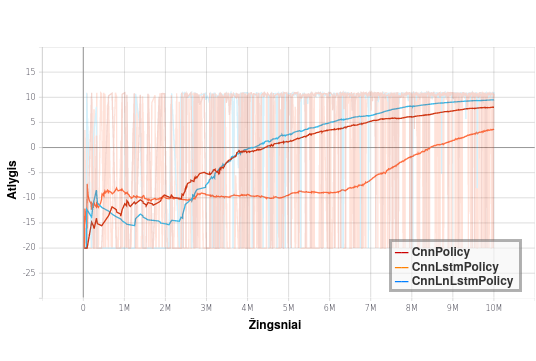
\includegraphics[scale=0.75]{img/graphs/policies}
		\caption{Agento mokymosi procesas su skirtingomis strategijomis. Tyrimai atlikti paprastoje Sokoban žaidimo aplinkoje, t.y. \(7 \times 7\) dydžio su viena dėže kambariai. Raudona linija -- A2C algoritmas naudojantis \code{CnnPolicy} strategija; oranžinė linija -- A2C algoritmas naudojantis \code{CnnLstmPolicy} strategija; mėlyna linija -- A2C algoritmas naudojantis \code{CnnLnLstmPolicy} strategija.}
		\label{img:policies_graph}
	\end{figure}
}
\subsubsection{Antros eksperimento dalies: geriausio algoritmo ieškojimo rezultatai}
{
	Paveikslėlyje~\ref{img:algorithms_graph} atvaizduoti agentų mokymo procesų su skirtingais algoritmais rezultatai. Kaip ir prognozuota, visi trys algoritmai pasiekia panašaus efektyvumo rezultatus, tačiau visiems šiems algoritmams prireikė skirtingo laiko žingsnių skaičiaus. ACER pasiekia optimalius rezultatus po \(3\cdot10^6\) žingsnių, PPO2 panašius rezultatus pasiekia apie \(4\cdot10^6\) žingsnyje, o A2C prireikia visų testavimo žingsnių (\(10^7\)) pasiekti tuos pačius rezultatus.\par
	Nors ACER mokėsi efektyviausiai žingsnių atžvilgiu, mokymui nustatyti \(10^7\) žingsnių užtruko  beveik \(10\) valandų, kai PPO2 užtrunka \(8\), o A2C -- \(6\) valandas (paveikslėlis~\ref{img:algorithms_time_graph}).
	
	\begin{figure}[H]
		\centering
		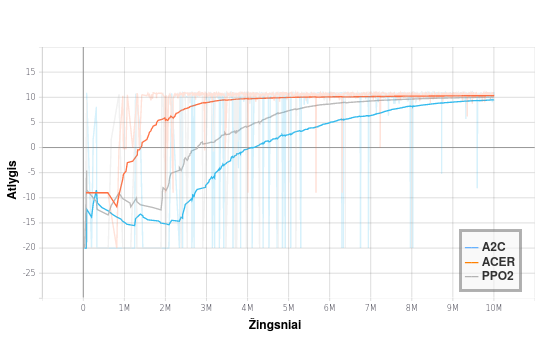
\includegraphics[scale=0.75]{img/graphs/algorithms}
		\caption{Agento mokymosi procesas su skirtingais algoritmais. Tyrimai atlikti paprastoje Sokoban žaidimo aplinkoje, t.y. \(7 \times 7\) dydžio su viena dėže kambariai. Mėlyna linija -- A2C algoritmas naudojantis \code{CnnLnLstmPolicy} strategija; oranžinė linija -- ACER algoritmas naudojantis \code{CnnLnLstmPolicy} strategija; pilka linija -- PPO2 algoritmas naudojantis \code{CnnLnLstmPolicy} strategija.}
		\label{img:algorithms_graph}
	\end{figure}
	\begin{figure}[H]
		\centering
		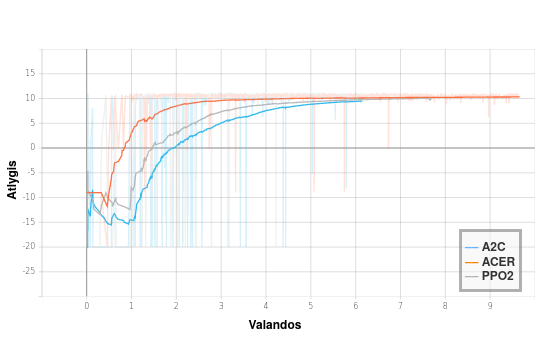
\includegraphics[scale=0.75]{img/graphs/algorithms_time}
		\caption{Agento mokymosi procesas su skirtingais algoritmais, laike. Tyrimai atlikti paprastoje Sokoban žaidimo aplinkoje, t.y. \(7 \times 7\) dydžio su viena dėže kambariai. Mėlyna linija -- A2C algoritmas naudojantis \code{CnnLnLstmPolicy} strategija; oranžinė linija -- ACER algoritmas naudojantis \code{CnnLnLstmPolicy} strategija; pilka linija -- PPO2 algoritmas naudojantis \code{CnnLnLstmPolicy} strategija.}
		\label{img:algorithms_time_graph}
	\end{figure}
}
\subsubsection{Trečios eksperimento dalies: mokymo žinių perdavimo naudos tyrimo rezultatai}
{
	Paveikslėlyje~\ref{img:a2c_completions} atvaizduoti A2C agentų mokymo procesų rezultatai. Bazinio modelio mokymas buvo nutrauktas po \(4,5 \cdot 10^7\) žingsnių ir \(50\) valandų, dėl mokymosi progreso nebuvimo. Tokie pat rezultatai buvo užfiksuoti su ACER algoritmu (paveikslėlis~\ref{img:acer_completions}), kurio bazinio modelio mokymas buvo nutrauktas po \(3,5 \cdot 10^7\) ir \(48\) valandų. PPO2 (paveikslėlis~\ref{img:ppo2_completions}) kita vertus, mokėsi ir su sudėtinga aplinka, tačiau mokymas buvo nutrauktas po \(4,8 \cdot 10^7\) žingsnių ir \(70\) valandų, dėl nuolatos lėtėjančio mokymo proceso.\par
	
	Nutraukus bazinių modelių mokymą, buvo pradėta mokyti modelius su paprastesne Sokoban žaidimo aplinka, tačiau didesnio (nei pirmoje ir antroje eksperimento dalyse) ploto kambariais. Pastebėta, kad ACER algoritmas, nors rodė gerus rezultatus antroje eksperimento dalyje, naujame teste laiko atžvilgiu pasirodė labai panašiai kaip A2C. Abu algoritmai apmokant agentą užtruko apie \(37\) valandas, o PPO2 užtruko tik \(22\) valandas, iki kol buvo pasiekta \(90\%\) iteracijos išspręstų kambarių dalis (lentelė~\ref{tab:all_results}, papunktis~\ref{subsubsubsec:sokoban_prepare}).\par
	
	Apmokius agentus su Sokoban aplinkomis, kuriose žaidėjas turėjo išspręsti galvosūkį tik su viena dėže, agento svoriai buvo perkelti į naują agentą, kuris tęsė mokymą ant sudėtingesnės aplinkos, su dviem dėžėmis. Pradžioje (paveikslėlis~\ref{img:a2c_completions}), visų naujų agentų išspręstų kambarių kiekis, natūraliai, nukrito iki beveik nulio. Tačiau PPO2 ir A2C pakankamai greitai pradėjo mokytis naujoje aplinkoje ir pasiekė eigoje minėtus kriterijus per \(30\) ir \(68\) valandas atitinkamai (A2C lėtesnis). ACER nepradėjo mokytis ir po \(36\) valandų, mokymas buvo nutrauktas. PPO2 agentas pradėjo mokytis anksčiau, bet reliatyviai greitai sulėtėjo iki stabdymo kriterijaus reikšmės ir pasiekė tik apie \(55\%\) kambarių išsprendimo dalį, kita vertus, A2C nors mokėsi lėčiau, tačiau tai atliko stabiliau ir pasiekė virš \(70\%\) galvosūkių su dviem dėžėmis išsprendimo dalį (lentelė~\ref{tab:all_results}, papunktis~\ref{subsubsubsec:sokoban_prepare}).
	
	\begin{figure}[H]
		\centering
		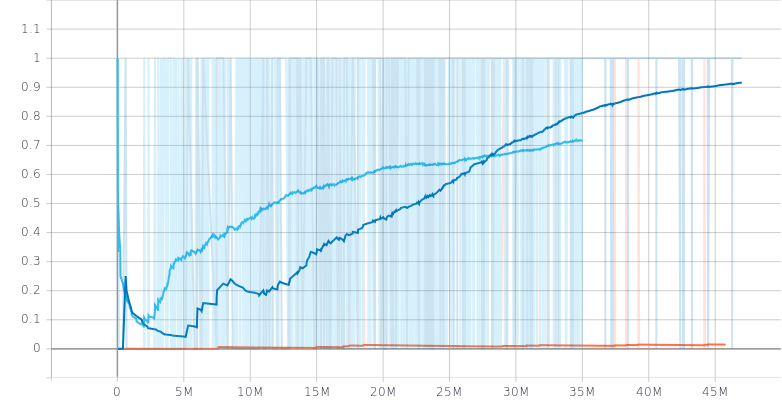
\includegraphics[scale=0.75]{img/graphs/a2c_completions}
		\caption{Agento mokymosi procesas su A2C algoritmu ir žinių perdavimu. Tyrimai atliekami Sokoban žaidimo aplinkoje su \(10 \times 10\) dydžio kambariais. Raudona linija -- A2C algoritmo mokymas kambariuose su viena dėže; mėlyna linija -- A2C algoritmo mokymas kambariuose su dviem dėžėmis; rožinė linija -- A2C algoritmo mokymas dviejų dėžių kambariuose su perduotomis žiniomis iš mokymosi su viena dėže.}
		\label{img:a2c_completions}
	\end{figure}
	\begin{figure}[H]
		\centering
		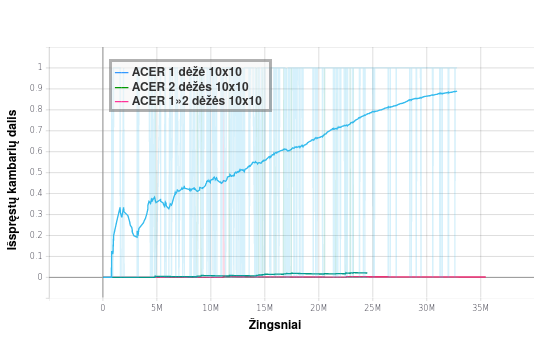
\includegraphics[scale=0.75]{img/graphs/acer_completions}
		\caption{Agento mokymosi procesas su ACER algoritmu ir žinių perdavimu. Tyrimai atliekami Sokoban žaidimo aplinkoje su \(10 \times 10\) dydžio kambariais. Mėlyna linija -- ACER algoritmo mokymas kambariuose su viena dėže; žalia linija -- ACER algoritmo mokymas kambariuose su dviem dėžėmis; rožinė linija -- ACER algoritmo mokymas dviejų dėžių kambariuose su perduotomis žiniomis iš mokymosi su viena dėže.}
		\label{img:acer_completions}
	\end{figure}
	\begin{figure}[H]
		\centering
		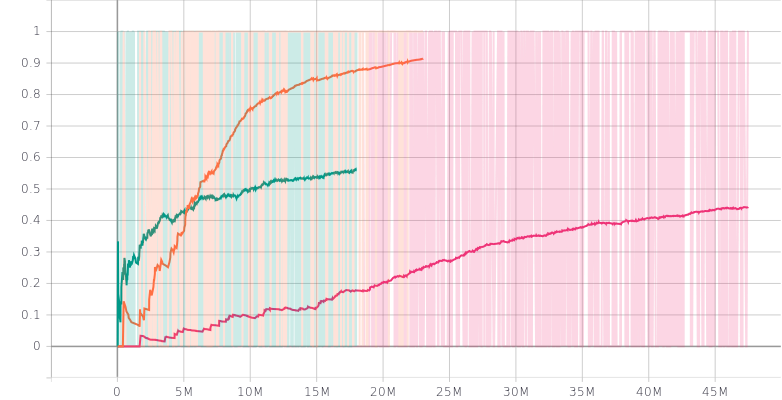
\includegraphics[scale=0.75]{img/graphs/ppo2_completions}
		\caption{Agento mokymosi procesas su PPO2 algoritmu ir žinių perdavimu. Tyrimai atliekami Sokoban žaidimo aplinkoje su \(10 \times 10\) dydžio kambariais. Mėlyna linija -- PPO2 algoritmo mokymas kambariuose su viena dėže; žalia linija -- PPO2 algoritmo mokymas kambariuose su dviem dėžėmis; pilka linija -- PPO2 algoritmo mokymas dviejų dėžių kambariuose su perduotomis žiniomis iš mokymosi su viena dėže.}
		\label{img:ppo2_completions}
	\end{figure}
}
\subsection{Eksperimento apibendrinimas ir išvados}
{
	Eksperimentas parodė, kad pritaikant Stable Baselines (punktas~\ref{subsubsec:stable-baselines}) algoritmų (A2C, ACER ir PPO2) implementacijas su numatytaisiais hiper-parametrais ir kitais nustatymais, Sokoban žaidimo agento mokymui, geriausias pasirinkimas iš tirtųjų  yra \code{CnnLnLstmPolicy} strategija (lentelė~\ref{tab:all_results}). Kadangi tyrimai atlikti su mažu (\(7 \time 7\)) Sokoban žaidimo aplinkos kambariu ir paprastomis sąlygomis (1 dėžė per kambarį), yra tikimybė, jog kitokios kambario specifikacijos rodytų kitokius rezultatus. Tačiau, jei mokomas paprastas Sokoban žaidimo agentas, \code{CnnPolicy} ir \code{CnnLnLstmPolicy} yra geros strategijos.\par
	
	Algoritmų mokymo palyginimas naudojant paprastą Sokoban žaidimo aplinką parodė, kad ACER ir PPO2 algoritmai mokosi greičiau nei A2C algoritmas žingsnių atžvilgiu. Tačiau šis tyrimas buvo atliktas su paprasta aplinka. Vėlesniuose tyrimuose buvo pastebėta, kad ACER algoritmas, kuris pasirodė geriausiai paprastos aplinkos mokyme, visiškai nesimoko sudėtingesnėje ir didesnėje aplinkoje, bent su autorių numatytaisiais nustatymais ir testuota Sokoban aplinka. Todėl, jei yra mokomas agentas paprastoje Sokoban žaidimo aplinkoje, ACER algoritmas yra geriausias pasirinkimas.\par
	
	Sokoban žaidimo agentas naudojantis PPO2 algoritmą parodė gerus rezultatus tiek paprastos aplinkos apmokyme, tiek sudėtingos. Taip pat, PPO2 buvo vienintelis algoritmas, kuris (nors ir lėtai), bet mokėsi sudėtingoje Sokoban žaidimo aplinkoje be žinių perdavimo. PPO2 agentas, lyginant su kitais tirtais, greičiausiai pasiekė mokymo kriterijus (daugiau nei \(90\%\) išspręstų kambarių dalis) sudėtingoje aplinkoje. Dėl to, mokant Sokoban žaidimo agentą be žinių perdavimo su didesniais (\(10 \times 10\)) ar sudėtingesniais (dvi dėžės) kambariais, geriausias pasirinkimas yra PPO2 algoritmas. \par
	 
	Labiausiai eksperimento metu pasižymėjo Sokoban žaidimo agentai su A2C algoritmu. Nors šie agentai neparodė geriausių rezultatų lyginant su ACER ir PPO2 algoritmu paprastoje Sokoban žaidimo aplinkoje, jų mokymosi rezultatai buvo stabiliausi sudėtingoje aplinkoje. A2C agentai, iš visų tirtų algoritmų, pasiekė aukščiausią Sokoban galvosūkių su dviem dėžėm išsprendimo procentą (\(72\%\)) prieš pasiekdami sustabdymo kriterijus. Nors bandant apmokyti su ta pačia aplinka nuo pradžių, agentas nerodė jokio progreso. Tai parodė, kad žinių perdavimas Sokoban žaidimo agentui paremtu A2C algoritmu, yra naudingas ir padeda agentui pasiekti aukštesnių išsprendimo rezultatų.\par
	
	Žinių perdavimas padėjo ne tik A2C, bet ir PPO2 algoritmui. PPO2 algoritmo Sokoban žaidimo agentas su žinių perdavimu pasiekė aukštesnius rezultatus ir daug greičiau nei be: agentas be žinių perdavimo užtruko \(70\) valandų ir pasiekė \(44\%\), agentai apmokyti su paprastesne aplinka ir perduotomis žiniomis užtruko bendrai \(53\) valandas ir pasiekė \(56\%\) išsprendimo procentą (papunktis~\ref{subsubsubsec:sokoban_prepare}).
	
	\begin{longtable}[H]{ccccccccc}
		\caption{Eksperimento metu atlikti mokymai. Dėžės skaičiai su rodyklėmis žymi mokymosi žinių perdavimą.}
		\label{tab:all_results} \\
		\toprule
		\multicolumn{1}{c}{\rotatebox[origin=l]{90}{\textbf{\begin{tabular}[l]{@{}l@{}}Algoritmas ir\\ strategija\end{tabular}}}} & \multicolumn{1}{c}{\rotatebox[origin=l]{90}{\textbf{\begin{tabular}[l]{@{}l@{}}Kambarių\\ dydis\end{tabular}}}} & \multicolumn{1}{c}{\rotatebox[origin=l]{90}{\textbf{\begin{tabular}[l]{@{}l@{}}Dėžių\\ skaičius\end{tabular}}}} & \multicolumn{1}{c}{\rotatebox[origin=l]{90}{\textbf{\begin{tabular}[l]{@{}l@{}}Mokymosi\\ laikas\end{tabular}}}} & \multicolumn{1}{c}{\rotatebox[origin=l]{90}{\textbf{\begin{tabular}[l]{@{}l@{}}Mokymosi\\ žingsniai (\(10^7\))\end{tabular}}}} & \multicolumn{1}{c}{\rotatebox[origin=l]{90}{\textbf{\begin{tabular}[l]{@{}l@{}}Mokymosi\\ atlygis\end{tabular}}}} & \multicolumn{1}{c}{\rotatebox[origin=l]{90}{\textbf{\begin{tabular}[l]{@{}l@{}}Išsprendimo\\ procentas\end{tabular}}}} \\
		\midrule
		\endhead
		%
		\begin{tabular}[l]{@{}c@{}}A2C \\ \code{CnnPolicy} \end{tabular} & \(7 \times 7\) & \(1\) & \begin{tabular}[l]{@{}c@{}} 5 val. \\ 18 min. \end{tabular} & \(1\) & \(8,02\) & -- \\
		\rowcolor[HTML]{EFEFEF} 
		\begin{tabular}[l]{@{}c@{}}A2C \\ \code{CnnLstmPolicy} \end{tabular} & \(7 \times 7\) & \(1\) & \begin{tabular}[l]{@{}c@{}} 4 val. \\ 41 min. \end{tabular} & \(1\) & \(3,67\) & -- \\
		\begin{tabular}[l]{@{}c@{}}A2C \\ \code{CnnLnLstmPolicy} \end{tabular} & \(7 \times 7\) & \(1\) & \begin{tabular}[l]{@{}c@{}} 6 val. \\ 8 min. \end{tabular} & \(1\) & \(9,49\) & -- \\
		\rowcolor[HTML]{EFEFEF} 
		\begin{tabular}[l]{@{}c@{}}ACER \\ \code{CnnLnLstmPolicy} \end{tabular} & \(7 \times 7\) & \(1\) & \begin{tabular}[l]{@{}c@{}} 9 val. \\ 39 min.\end{tabular}  & \(1\) & \(10,06\) & -- \\
		\begin{tabular}[l]{@{}c@{}}PPO2 \\ \code{CnnLnLstmPolicy} \end{tabular} & \(7 \times 7\) & \(1\) & \begin{tabular}[l]{@{}c@{}} 7 val. \\ 38 min. \end{tabular} & \(1\) & \(-9,60\) & -- \\
		\rowcolor[HTML]{EFEFEF} 
		\begin{tabular}[l]{@{}c@{}}A2C \\ \code{CnnLnLstmPolicy} \end{tabular} & \(10 \times 10\) & \(1\) & \begin{tabular}[l]{@{}c@{}} 67 val. \\ 18 min. \end{tabular} & \(4,7\) & \(8,52\) & \(92\%\) \\
		\begin{tabular}[l]{@{}c@{}}A2C \\ \code{CnnLnLstmPolicy} \end{tabular} & \(10 \times 10\) & \(2\) & \begin{tabular}[l]{@{}c@{}} 50 val. \\ 12 min. \end{tabular} & \(4,6\) & \(10,32\) & \(1\%\) \\
		\rowcolor[HTML]{EFEFEF} 
		\begin{tabular}[l]{@{}c@{}}A2C \\ \code{CnnLnLstmPolicy} \end{tabular} & \(10 \times 10\) & \(1 \rightarrow 2\) & \begin{tabular}[l]{@{}c@{}} 37 val. \\ 4 min. \end{tabular} & \(3,5\) & \(4,43\) & \(72\%\) \\
		\begin{tabular}[l]{@{}c@{}}ACER \\ \code{CnnLnLstmPolicy} \end{tabular} & \(10 \times 10\) & \(1\) & \begin{tabular}[l]{@{}c@{}} 38 val. \\ 27 min. \end{tabular} & \(3,3\) & \(8,74\) & \(92\%\) \\
		\rowcolor[HTML]{EFEFEF} 
		\begin{tabular}[l]{@{}c@{}}ACER \\ \code{CnnLnLstmPolicy} \end{tabular} & \(10 \times 10\) & \(2\) & \begin{tabular}[l]{@{}c@{}} 35 val. \\ 47 min. \end{tabular} & \(2,5\) & \(-9,64\) & \(2\%\) \\
		\begin{tabular}[l]{@{}c@{}}ACER \\ \code{CnnLnLstmPolicy} \end{tabular} & \(10 \times 10\) & \(1 \rightarrow 2\) & \begin{tabular}[l]{@{}c@{}} 48 val. \\ 5 min. \end{tabular} & \(3,5\) & \(-9,85\) & \(0\%\) \\
		\rowcolor[HTML]{EFEFEF} 
		\begin{tabular}[l]{@{}c@{}}PPO2 \\ \code{CnnLnLstmPolicy} \end{tabular} & \(10 \times 10\) & \(1\) & \begin{tabular}[l]{@{}c@{}} 22 val. \\ 58 min. \end{tabular} & \(2,3\) & \(8,38\) & \(91\%\) \\
		\begin{tabular}[l]{@{}c@{}}PPO2 \\ \code{CnnLnLstmPolicy} \end{tabular} & \(10 \times 10\) & \(2\) & \begin{tabular}[l]{@{}c@{}} 69 val. \\ 48 min. \end{tabular} & \(4,7\) & \(-0,34\) & \(44\%\)\\
		\rowcolor[HTML]{EFEFEF} 
		\begin{tabular}[l]{@{}c@{}}PPO2 \\ \code{CnnLnLstmPolicy} \end{tabular} & \(10 \times 10\) & \(1 \rightarrow 2\) & \begin{tabular}[l]{@{}c@{}} 29 val. \\ 27 min. \end{tabular} & \(1,8\) & \(0,16\) & \(56\%\) \\
		\bottomrule
	\end{longtable}
}
\sectionnonum{Rezultatai}
{
	Šio darbo metu buvo pasiektas \textbf{tikslas} -- palyginti skatinamojo mokymosi algoritmai, nustatyti efektyviausi algoritmai ir strategijos Sokoban žaidimui skirtingose situacijose.
	
	Įgyvendinti darbui iškelti \textbf{uždainiai}:
	\begin{enumerate}
		\item Atlikta skatinamojo mokymosi algoritmų analizė, parinkta Stable Baselines RL biblioteka ir atrinkti trys potencialūs algoritmai Sokoban žaidimo agento mokymui: A2C, ACER ir PPO2.
		
		\item Paruošta eksperimentinė Sokoban žaidimo aplinka. Gym-Sokoban OpenAI Gym aplinkai suprogramuoti pagalbiniai dekoratoriai. Mokymui paruoštos programos ir iškviečiamos funkcijos, mokymosi stebėjimui.
		
		\item Atliktas eksperimentas, nustatyta geriausia, naudotos RL bibliotekos strategija Sokoban žaidimo agento valdymui.
		
		\item Eksperimentiškai palygintos Stable Baselines RL algoritmų implementacijos su numatytaisiais nustatymais: A2C, ACER ir PPO2. Palyginimui naudota mažiausia įmanoma Sokoban žaidimo aplinka: \(7 \times 7\) kambario dydis su viena dėže per kambarį.
		
		\item Panaudotas žinių perdavimas, apmokyti Sokoban žaidimo agentai veikti sudėtingesnėse aplinkose, t.y. \(10 \times 10\) kambario dydžio su dviem dėžėmis. Dar sudėtingesnės aplinkos nebuvo bandomos, dėl labai ilgo apmokymo laiko.
	\end{enumerate}
}
\sectionnonum{Išvados}
{
	Šiame darbe atlikti eksperimentai leidžia daryti tokias išvadas:
	\begin{enumerate}
		\item Eksperimentiškai palyginus Stable Baselines RL bibliotekos strategijas nustatyta, kad \code{CnnLnLstmPolicy} strategija yra geriausia Sokoban žaidimo agento mokymui lyginant su \code{CnnPolicy} ir \code{CnnLstmPolicy} (paveikslėlis~\ref{img:policies_graph}, lentelė~\ref{tab:all_results}). Antra pagal gerumą strategija yra \code{CnnPolicy}, ji pasiekia \(15\%\) mažesnį tikslumą, lyginant su \code{CnnLnLstmPolicy}, Sokoban žaidimo aplinkoje su viena dėže ir \(7 \times 7\) kambario dydžiu.
		
		\item Atlikus lyginamuosius eksperimentus, nustatyta, kad Sokoban žaidimo agentas, naudojantis ACER algoritmą (su numatytaisiais parametrais) yra geriausiai besimokantis mažiausioje Sokoban žaidimo (\(7 \times 7\) kambario dydžio su viena dėže) aplinkoje lyginant su A2C ir PPO2 algoritmais (paveikslėlis~\ref{img:algorithms_graph}, lentelė~\ref{tab:all_results}), tačiau tai jis padaro per ilgiausią laiko tarpą.
		
		\item Palyginus Sokoban žaidimo agentų mokymosi rezultatus naudojant ir nenaudojant mokymosi žinių perdavimą sudėtingesnėje (\(10 \times 10\) kambario dydžio su dviem dėžėmis) aplinkoje, nustatyta, kad agentas naudojantis mokymosi žinių perdavimą pasiekia geresnius rezultatus per trumpesnį laiką ir mažesnį žingsnių skaičių dviem iš trijų tirtų atvejų:
		\begin{enumerate}
			\item Eksperimento metu gauti rezultatai rodo, kad naudojant ACER algoritmą (su numatytaisiais parametrais) sudėtingesnės (\(10 \times 10\) kambario dydžio su dviem dėžėmis) Sokoban žaidimo aplinkos mokymui, geri rezultatai per priimtiną laiką negaunami, nepriklausomai ar mokymosi žinių perdavimas yra taikomas ar ne (paveikslėlis~\ref{img:acer_completions}, lentelė~\ref{tab:all_results}).
			
			\item Mokinant PPO2 algoritmo (su numatytaisiais parametrais) agentą su mokymosi žinių perdavimu, gauti geresni rezultatai. Nors PPO2 agentas mokėsi sudėtingoje aplinkoje be žinių perdavimo (pasiekė \(44\%\) kambarių išsprendimo procentą per duotą \(70\) valandų mokymosi laiką), agentas su žinių perdavimu pasiekė aukštesnius rezultatus (\(56\%\) kambarių išsprendimo procentą) per trumpesnį bendrą (pirminio agento ir perėmusio žinias agento) mokymosi laiką (\(53\) valandas).
			
			\item A2C (su numatytaisiais parametrais) agentas su žinių perdavimu parodė geriausius rezultatus ir pasiekė \(72\%\) kambarių išsprendimo procentą (lentelė~\ref{tab:all_results}). A2C agentas be žinių perdavimo nesimokė ir per priimtiną mokymosi laiką nepakilo aukščiau \(1\%\) išspręstų kambarių.
		\end{enumerate}
	\end{enumerate}
}
\printbibliography[heading=bibintoc] 

\sectionnonum{Santrumpos}
{
	Darbe naudojamų \textbf{santrumpų paaiškinimai}:
	\begin{itemize}
		\item \textbf{A2C} -- (\textit{angl. Advantage Actor-Critic}) pranašumo aktoriaus-kritiko algoritmas.
		\item \textbf{A3C} -- (\textit{angl. Asynchronous Advantage Actor-Critic}) asinchroninis pranašumo aktoriaus-kritiko algoritmas.
		\item \textbf{ACER} -- (\textit{angl. Actor-Critic with Experience Replay}) aktorius-kritiko su patirties pakartojimu algoritmas.
		\item \textbf{ANN} -- (\textit{angl. Artificial Neural Network}) dirbtinis neuroninis tinklas.
		\item \textbf{API} -- (\textit{angl. Application Programming Interface}) aplikacijų programavimo sąsaja.
		\item \textbf{CNN} -- (\textit{angl. Convolutional Neural Network}) konvoliucinis neuroninis tinklas.
		\item \textbf{CPU} -- (\textit{angl. Central Processing Unit}) centrinis procesorius.
		\item \textbf{DNN} -- (\textit{angl. Deep Neural Network}) gilusis neuroninis tinklas.
		\item \textbf{GPU} -- (\textit{angl. Graphics Processing Unit}) grafinis procesorius.
		\item \textbf{LSTM} -- (\textit{angl. Long Short-Term Memory}) ilgos trumpalaikės atminties modelis.
		\item \textbf{LTU} -- (\textit{angl. Linear Treshold Unit}) linijinis slenksčio vienetas.
		\item \textbf{MDP} -- (\textit{angl. Markov Decision Processes}) Markovo sprendimo priėmimo procesai.
		\item \textbf{ML} -- (\textit{angl. Machine Learning}) mašininis mokymasis.
		\item \textbf{MLP} -- (\textit{angl. Multi-Layer Perceptrons}) daugiasluoksnis perceptronas.
		\item \textbf{PG} -- (\textit{angl. Policy Gradient}) strategijos gradientas.
		\item \textbf{PPO} -- (\textit{angl. Proximal Policy Optimization}) proksimalinis strategijos optimizavimo algoritmas.
		\item \textbf{RGB} -- (\textit{angl. Red Green Blue colour model}) raudona, žalia, mėlyna spalvos.
		\item \textbf{RL} -- (\textit{angl. Reinforcement Learning}) skatinamasis mokymas.
		\item \textbf{RNN} -- (\textit{angl. Recurrent Neural Network}) rekurentinis neuroninis tinklas.
		\item \textbf{VSC} -- (\textit{angl. Version-Control System}) versijų tvarkymo sistema.
	\end{itemize}
}

\appendix

\section{Stable Baselines skatinamojo mokymosi bibliotekos algoritmų A2C, ACER, PPO2 implementacijų numatytosios hiper-parametrų reikšmės}\label{app:algorithms}
{
	Bakalauro darbo metu yra naudojamos Stable Baselines skatinamojo mokymosi bibliotekos algoritmų implementacijos su jų autorių numatytosiomis hiper-parametrų reikšmėmis, kurios yra nurodytos lentelėje~\ref{tab:algorithm_defaults}.
	
	\begin{table}[H]
		\centering
		\caption{A2C, ACER, PPO2 algoritmų implementacijų numatytosios hiper-parametrų reikšmės}
		\label{tab:algorithm_defaults}
		\begin{tabular}{lccc}
			\toprule
			\multicolumn{1}{c}{\textbf{Hiper-parametro}} & \multicolumn{3}{c}{\textbf{Algoritmai}} \\
			\multicolumn{1}{c}{\textbf{pavadinimai}} & \textbf{A2C} & \textbf{ACER} & \textbf{PPO2} \\
			\midrule
			\code{gamma} & \(0,99\) & \(0,99\) & \(0,99\) \\
			\rowcolor[HTML]{EFEFEF} 
			\code{n\_steps} & \(5\) & \(20\) & \(128\) \\
			\code{vf\_coef} & \(0,25\) & -- & \(0,5\) \\
			\rowcolor[HTML]{EFEFEF} 
			\code{q\_coef} & -- & \(0,5\) & -- \\
			\code{ent\_coef} & \(0,01\) & \(0,01\) & \(0,01\) \\
			\rowcolor[HTML]{EFEFEF} 
			\code{max\_grad\_norm} & \(0,5\) & \(10\) & \(0,5\) \\
			\code{learning\_rate} & \(7 \cdot 10^{-4}\) & \(7 \cdot 10^{-4}\) & \(2,5 \cdot 10^{-4}\) \\
			\rowcolor[HTML]{EFEFEF} 
			\code{alpha} & \(0,99\) & \(0,99\) & -- \\
			\code{momentum} & \(0,0\) & -- & -- \\
			\rowcolor[HTML]{EFEFEF} 
			\code{epsilon} & \(10^{-5}\) & -- & -- \\
			\code{lr\_schedule} & -- & \code{'linear'} & -- \\
			\rowcolor[HTML]{EFEFEF} 
			\code{rprop\_alpha} & -- & \(0,99\) & -- \\
			\code{rprop\_epsilon} & -- & \(10^{-5}\) & -- \\
			\rowcolor[HTML]{EFEFEF} 
			\code{buffer\_size} & -- & \(5000\) & -- \\
			\code{replay\_ratio} & -- & \(4\) & -- \\
			\rowcolor[HTML]{EFEFEF} 
			\code{replay\_start} & -- & \(1000\) & -- \\
			\code{correction\_term} & -- & \(10,0\) & -- \\
			\rowcolor[HTML]{EFEFEF} 
			\code{lam} & -- & -- & \(0,95\) \\
			\code{nminibatches} & -- & -- & \(4\) \\
			\rowcolor[HTML]{EFEFEF} 
			\code{noptepochs} & -- & -- & \(4\) \\
			\code{cliprange} & -- & -- & \(0,2\) \\
			\bottomrule
		\end{tabular}
	\end{table}
}
\section{Sokoban aplinkai pagal OpenAI Gym principus parašytas programinis kodas}\label{app:wrappers}
{
	Čia apibrėžti trys papildomi dekoratoriai paremti OpenAI Gym \code{Wrapper} aplinkos dekoratoriaus interfeisu (papunktis~\ref{subsubsubsec:gym}). \code{ActionWrapper} limituoja leidžiamų atlikti veiksmų sritį. \code{ExposeCompletedEnvironments} naudojamas su bakalauro darbo metu parašytomis per-kvietimo funkcijomis. Šis dekoratorius, padaro sėkmingai užbaigtų aplinkų skaitinę reikšmę pasiekiamą iš išorės. \code{CombinedWrappers} pagalbinis dekoratorius, leidžiantis lengvai sukurti aplinkos objektą su keliais dekoratoriais iš karto.
	\lstinputlisting[language=Python]{code/my_wrappers.py}
}
\section{Modelio mokymo programinis kodas A2C, ACER ir PPO2 algoritmams bei CnnPolicy, CnnLstmPolicy ir CnnLnLstmPolicy strategijoms}\label{app:strategies}
{
	Originaliai, programa parašyta naudojantis Jupyter Notebook aplinka. Čia pateikiamas programos atitikmuo Python skripto failu. Programa leidžia nurodyti tiriamą algoritmą (punktas~\ref{subsubsec:algorithms}) bei strategiją (punktas~\ref{subsubsec:policies}). Nustatoma modelio aplinka: \(7 \times 7\) dydžio kambarys, viena dėžė bei penki galimi veiksmai. Nurodytas modelis yra apmokomas \(10^7\) žingsnių ir išsaugomas į failą. Mokymosi procesas yra stebimas naudojantis TensorBoard, iš kurio yra gaunami duomenys analizei.
	\lstinputlisting[language=Python]{code/strategies.py}
}
\section{Modelio mokymo su žinių perdavimu programinis kodas}\label{app:curriculum}
{
	Python programa apmokanti nurodyto algoritmo (punktas~\ref{subsubsec:algorithms}) ir \code{CnnLnLstmPolicy} strategijos (papunktis~\ref{subsubsubsec:cnnlnlstmpolicy}) modelį su nurodytais pradiniais aplinkos sudėtingumo nustatymais:  \(10 \times 10\) dydžio kambarys, viena dėžė bei penki galimi veiksmai. Mokoma iki kol nurodyti mokymo kriterijai yra pasiekiami: mokymas trunka bent \(5\) iteracijas, paskutinės iteracijos išspręstų kambarių dalis yra bent \(50\%\), paskutinių \(5\) iteracijų vidurkio ir paskutinės iteracijos išspręstų kambarių absoliutus skirtumas yra žemiau \(1\%\) arba paskutinės iteracijos išspręstų kambarių dalis yra daugiau nei \(90\%\). Kai kriterijai pasiekiami, modeliui duodama sudėtingesnė aplinka ir mokymas yra kartojamas iki nurodyto sudėtingumo.
	\lstinputlisting[language=Python]{code/curriculum_learning.py}
}
\end{document}
